        \section{Linear Transformations}
        Now that we have set the stage for vectors and the products between them, we would like to investigate how we can transform these vectors.  Specifically, we will first care about functions that are \emph{linear}.  These will be functions that stretch and rotate vectors and possibly change dimension all while leaving the origin alone.
        
        \begin{df}{Linear Transformation}{linear_transformation}
        A \boldgreen{linear transformation} \index{linear!transformation} is a function
        \[
        T\colon \R^n \to \R^m
        \]
        that satisfies the following requirements:
        \begin{enumerate}[(i)]
            \item $T(\vecu+\vecv)=T(\vecu)+T(\vecv)$,
            \item $T(\alpha \vecv)=\alpha T(\vecv)$,
            \item $T(\zerovec)=\zerovec$.
        \end{enumerate}
        Note that requirement (iii) follows from (i) and (ii), but it is something that is easy to check, so we place it here as well.
        \end{df}
        
        \begin{remark}
        When writing transformations of vectors, we often omit the extra parentheses. That is, instead of
        \[
        T \left( \begin{pmatrix} x \\ y \\ z \end{pmatrix} \right),
        \]
        we will just put
        \[
        T \begin{pmatrix} x \\ y \\ z \end{pmatrix}.
        \]
        \end{remark}
        
        \begin{remark}
        These rules should seem similar to the properties of the derivative and integral.  We'll find that what we're building here will let us properly talk about derivatives in multiple dimensions.
        \end{remark}   
        
        \begin{ex}{Scaling is Linear}{sacaling_linear}
        Consider $T \colon \R^2 \to \R^2$ given by
        \[
        T\begin{pmatrix} x\\ y \end{pmatrix}
        = \begin{pmatrix} \alpha x\\ \beta y \end{pmatrix}.
        \]
        This transformation scales the $x$-component of our vector by $\alpha$ and scales the $y$-component by $\beta$.
        
        To see that this is linear, we just check that it satisfies the three necessary conditions.  First we will show (i). So, if we take two vectors
        \[
        \vecv_1 = \begin{pmatrix} x_1 \\ y_1 \end{pmatrix} \qquad \textrm{and} \qquad \vecv_2 = \begin{pmatrix} x_2 \\ y_2 \end{pmatrix},
        \]
        then we have
        \begin{align*}
        T\left( \vecv_1 + \vecv_2\right)&= T \left( \begin{pmatrix} x_1 \\ y_1 \end{pmatrix} + \begin{pmatrix} x_2 \\ y_2 \end{pmatrix} \right)\\
        &= T\left( \begin{pmatrix} x_1 + x_2 \\ y_1 + y_2 \end{pmatrix} \right)\\
        &= \begin{pmatrix} \alpha(x_1 + x_2) \\ \beta(y_1 + y_2)\end{pmatrix}\\
        &= \begin{pmatrix} \alpha x_1 + \alpha x_2 \\ \beta y_1 + \beta y_2 \end{pmatrix}\\
        &= \begin{pmatrix} \alpha x_1 \\ \beta y_1 \end{pmatrix} + \begin{pmatrix} \alpha x_2 \\ \beta y_2 \end{pmatrix} \\
        &= T(\vecv_1)+T(\vecv_2).
        \end{align*}
        
        Then for (ii), take $\vecv = x\xhat + y\yhat$ and we have
        \begin{align*}
            T(\mu \vecv)&=T\left(\mu \begin{pmatrix} x \\ y \end{pmatrix}\right)\\
            &=T\left( \begin{pmatrix} \mu x \\ \mu y \end{pmatrix}\right)\\
            &= \begin{pmatrix} \alpha \mu x \\ \beta \mu y \end{pmatrix}\\
            &= \mu \begin{pmatrix} \alpha x \\ \beta y \end{pmatrix}\\
            &= \mu T(\vecv).
        \end{align*}
        Since the qualities (i) and (ii) imply (iii), we don't necessarily need to check it. But, we can anyway. So we take
        \begin{align*}
            T(\zerovec)&= T\left(\begin{pmatrix} 0 \\ 0  \end{pmatrix}\right)\\
            &= \begin{pmatrix} \alpha \cdot 0 \\ \beta \cdot 0\end{pmatrix}\\
            &= \zerovec.
        \end{align*}
        So this function $T$ is indeed linear.
        \end{ex}
        
        \begin{exercise}
        Which of the following are linear transformations? Why or why not?
        \begin{enumerate}[(a)]
            \item $f\colon \R \to \R$ given by $f(x)=\lambda x$.
            \item $g\colon \R \to \R$ given by $g(x)=2x+1.$
            \item $h\colon \R \to \R$ given by $h(x)=x^2.$
            \item $T \colon \R^3 \to \R^3$ given by
            \[
            T \begin{pmatrix} x\\ y\\ z \end{pmatrix}  = \begin{pmatrix} y\\ x\\ z \end{pmatrix}.
            \]
        \end{enumerate}
        \end{exercise}
        
        % \begin{ex}{Dot Product is Linear}{dot_prod_linear}
        % If we choose a fixed vector $\mathbf{v}$, then the dot product of another vector $\mathbf{a}$ with $\mathbf{v}$ is itself an example of a linear transformation! It's also a good example of how the input dimension can differ from the output dimension.  Let us write $\textrm{Dot}_\mathbf{v}\colon \R^3 \to \R$ which is given by
        % \[
        % \textrm{Dot}_\mathbf{v}(\mathbf{a})=\mathbf{a}\cdot \mathbf{v}=a_xv_x+a_yv_y+a_zv_z.
        % \]
        % \end{ex}
        
        \begin{exercise}
        Pick a vector in the plane and draw a picture of the scaling transformation.
        \end{exercise}
        
        \begin{ex}{Rotation is Linear}{rot_linear}
        Consider the following linear transformation $T\colon \R^2 \to \R^2$ given by
        \[
        T\begin{pmatrix} x\\ y \end{pmatrix} 
        = \begin{pmatrix} x \cos \theta - y \sin \theta\\ x \sin \theta +y \cos \theta \end{pmatrix} = \begin{pmatrix} x'\\ y' \end{pmatrix}.
        \]
        This transformation rotates a vector by $\theta$ in the counter-clockwise direction. 
        \begin{figure}[H]
            \centering
            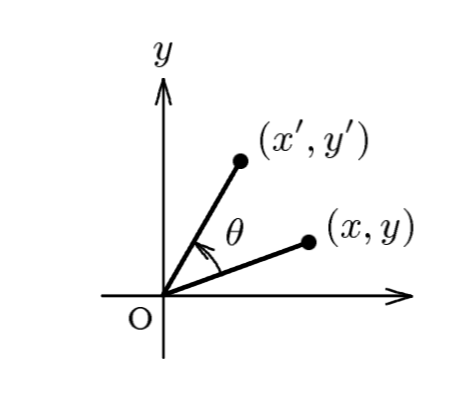
\includegraphics[width=.3\textwidth]{Figures/plane_rotation.png}
        \end{figure}
        \end{ex}
        
    \section{Matrix Representation of Linear Transformations}
        
        The salient fact of linear transformations is how we can represent them.  As it turns out, any linear transformation $T\colon \R^n \to \R^m$ can be written like:
        \[
        T\begin{pmatrix} x_1 \\ x_2 \\ \vdots \\ x_n \end{pmatrix}
        = \begin{pmatrix} y_1 \\ y_2 \\ \vdots \\ y_m \end{pmatrix},
        \]
        where 
        \begin{align*}
            y_1 &= a_{11} x_1 + a_{12} x_2 + a_{13} x_3 + \cdots + a_{1n} x_n\\
            y_2 &= a_{21} x_1 + a_{22} x_2 + a_{23} x_3 + \cdots + a_{2n} x_n\\
            y_3 &= a_{31} x_1 + a_{32} x_2 + a_{33} x_3 + \cdots + a_{3n} x_n\\
            \vdots\\
            y_m &= a_{m1} x_1 + a_{m2} x_2 + a_{m3} x_3 + \cdots + a_{mn} x_n.
        \end{align*}
        Hence, this arbitrary linear transformation is captured entirely by the \boldgreen{matrix} of numbers
        \[
        \begin{pmatrix}
        a_{11} & a_{12} & a_{13} & \cdots & a_{1n}\\
        a_{21} & a_{22} & a_{23} & \cdots & a_{2n}\\
        a_{31} & a_{32} & a_{33} & \cdots & a_{3n}\\
        \vdots & \vdots & \vdots & & \vdots \\
        a_{n1} & a_{n2} & a_{n3} & \cdots & a_{nm}
        \end{pmatrix}
        \]
        
        Now, our study moves to that of matrices since we have seen that matrices capture all that we need in order to describe linear transformations.  They aren't necessary to use, but they make computation and understanding a bit easier.  It turns out that we can also think of vectors as special cases of matrices, which makes the idea of studying matrices themselves all that much better. From here on out, we will restrict ourselves to matrix representations.  
        
        Often, one may be handed a linear transformation $T\colon \R^n \to \R^m$ as above. When one wants to represent $T$ as a matrix, we may put
        \[
        [T]=        \begin{pmatrix}
        a_{11} & a_{12} & a_{13} & \cdots & a_{1n}\\
        a_{21} & a_{22} & a_{23} & \cdots & a_{2n}\\
        a_{31} & a_{32} & a_{33} & \cdots & a_{3n}\\
        \vdots & \vdots & \vdots & & \vdots \\
        a_{n1} & a_{n2} & a_{n3} & \cdots & a_{nm}
        \end{pmatrix}.
        \]
        However, we will often just assume that a linear transformation is given as a matrix a priori.  As one continues to learn more linear algebra, it becomes clear why we wish to make this distinction, but for now this is alright.  In the sequel, we will care about understanding \emph{linear operators} which will not always have some matrix representation.
        
        \subsection{Matrix Algebra}
        Just as we did with vectors, we want to understand what we can do with these matrices algebraically.  These matrices must allow us to perform linear transformations.  Given that linear transformations are special types of functions, we also want to be able to compose linear functions as well.  All that we need will be captured in an algebraic way through matrix multiplication.  
        
        We will call a matrix with $n$-rows and $m$-columns an \textbf{$n\times m$-matrix} (read: $n$ by $m$ matrix).  These take the form:
        \[[A]=
        \begin{bmatrix}
        a_{11} & a_{12} & a_{13} & \cdots & a_{1n}\\
        a_{21} & a_{22} & a_{23} & \cdots & a_{2n}\\
        a_{31} & a_{32} & a_{33} & \cdots & a_{3n}\\
        \vdots & \vdots & \vdots & & \vdots \\
        a_{n1} & a_{n2} & a_{n3} & \cdots & a_{nm}
        \end{bmatrix}.
        \]
        We use a capital letter in brackets to denote a matrix. Each entry of the matrix will be given by a lowercase letter with subscripts $a_{ij}$.  The subscripts will tell you which row and column the entry is located. For example, $a_{25}$ would be the entry in the 2$^\textrm{nd}$ row and $5^\textrm{th}$ column.
        
        \begin{itemize}
            \item \textbf{Equality:} Matrices are equal if each entry is equal. That is, given $\matA$ and $\matB$, we say $\matA=\matB$ if $a_{ij}=b_{ij}$ for each pair $i,j$.  Clearly if these matrices are not the same ``shape" (meaning, they have a different number of rows or columns), then they cannot be the same.  Just as a 2-dimensional vector cannot be the same as a 3-dimensional one.  They are distinctly different objects.
            
            \item \textbf{Addition:} We can add matrices of the same shape.  We write $\matA+\matB=\matC$ and create the new matrix $\matC$ by adding the entries.  That is, $c_{ij}=a_{ij}+b_{ij}$.  
            
            \item \textbf{Scalar Multiplication:} We can also scale matrices.  We do this by scaling the entries.  So, if we have $\alpha \matA=\matB$, then we know the entries of $\matB$ are given by $b_{ij}=\alpha a_{ij}$.
            
            \item \textbf{Matrix Multiplication:} It is also possible to multiply two matrices together.  Recall that matrices are how we capture the information of a linear transformation. Matrix multiplication will capture the idea of composing two linear transformations. Consider two linear transformations
            \[
            A \colon \R^n \to \R^m \qquad \textrm{and} \qquad B \colon \R^m \to \R^p.
            \]
            Then we have that $[A]$ is an $m\times n$-matrix and $[B]$ is a $p\times m$ matrix.  We can create the composite linear transformation 
            \[
            B \circ A \colon \R^n \to \R^p,
            \]
            and hence we would like to understand how to represent this composite function with the two matrices $[A]$ and $[B]$. We define the matrix multiplication
            \[
            [B][A]=[C]
            \]
            to properly capture the composite linear transformation $A\circ B$. Hence, we can multiply matrices $\matA$ and $\matB$ if 
            \[
            \textrm{the number of columns of $\matA$}=\textrm{the number of rows of $\matB$}.
            \]
            If $\matA$ is an $m\times n$-matrix and $\matB$ is an $p\times m$-matrix, then $\matC=\matB \matA$ is an $m\times p$ matrix.  You can remember this helpful fact:
            \[
            (p\times \underbrace{m)\cdot (m}_{\textrm{the same}}\times n)
            \]
            and
            \[
            (\underbrace{p}\times m)\cdot (m\times \underbrace{n})
            \]      
            gives the dimensions of the resulting matrix.
            
            How we perform this matrix multiplication looks a bit ugly at first, but it ends up being slightly easier after digesting this a bit. We have that the components of $\matC=\matB \matA$ are
            \[
            c_{ij}=\sum_{k=1}^m b_{ik}a_{kj}.
            \]
            
            Let us take the example of letting $\matB$ be an $1\times n$-matrix and $\matA$ a $n\times 1$-matrix. Then
            \[
            [B][A]=
            \begin{bmatrix} b_{11} & b_{12} & \cdots & b_{1n}\end{bmatrix}
            \begin{bmatrix} a_{11}\\ a_{21} \\ \vdots \\ a_{n1}\end{bmatrix}=b_{11}a_{11}+b_{12}a_{21}+\cdots+b_{1n}a_{n1}=\sum_{k=1}^n b_{1k}a_{k1}.
            \]
            This is the dot product of two vectors!  As it turns out, we can decompose matrix multiplication into a bunch of dot products. 
            
            In general, if we look at the multiplication described above for the component $c_{ij}$, we can break this down as follows. Note that the $i$th row of a matrix $\matB$ is a vector with $m$ elements, the $j$th column of a matrix $\matA$ is a vector with $m$ elements, and the dot product of these two vectors gives the entry $c_{ij}$ of the matrix $\matB \matA=\matC$.
            \end{itemize}
            
            \begin{remark}
            This all means it is possible to take linear combinations of matrices as well!
            \end{remark}
            
            \begin{prop}{$n\times m$-Matrices Form a Vector Space}{matrix_vspace}
                Let $\mathcal{M}_{n\times m}$ be the set of all $m\times n$-matrices with real or complex entries. Then this set forms a vector space with the scalar multiplication and matrix addition described above.
            \end{prop}
            
            \begin{exercise}
                Show that the above proposition is true.
            \end{exercise}
            
            \begin{ex}{Multiplying Matrices}{multiplying_matrices}
            Let us multiply the following matrices:
            \[
            \matA=\begin{pmatrix} 2 & 0 & -3\\ 1&1&-2\end{pmatrix} \quad \matB=\begin{pmatrix} 2&3&4&1\\1&2&2&0\\0&-1&2&0\end{pmatrix}.
            \]
            Verify that you get
            \[
            \matA \matB=\begin{pmatrix} 4&9&2&2\\3&7&2&1\end{pmatrix}.
            \]
            \end{ex}
            
            \subsection{Properties of Matrix Multiplication}
            
            Matrices will behave in the following ways:
            \begin{itemize}
                \item \textbf{Associativity:} The order in which you choose to multiply matrices does not matter.  That is 
                \[\matA(\matB \matC)=(\matA \matB)\matC=\matA \matB \matC.\]
                \item \textbf{Distributivity:} We can multiply matrices over sums. That is
                \[
                \matA\left(\matB+\matC\right)=\matA \matB+\matA \matC.
                \]
                \item \textbf{(non)-Commutivity:} In general, we have
                \[
                \matA \matB\neq \matB \matA.
                \]
                However, there are certain types of matrices that do commute with each other.
            \end{itemize}
        
        Right now we have the ability to write linear transformations as matrices.  We can also multiply these matrices.  Keep in mind that this in some way mimics composing functions. In essence, we have entirely captured the functional behavior of linear spaces through matrices, since, we can realize vectors as special types of matrices as well.
        
        \section{Systems of Linear Equations}
        Often times we are handed a system of equations to solve.  In this case, we have more than one variable, and the same number of equations is required in order to determine values for these variables uniquely. For example, one may have three equations for the variables $x$, $y$, and $z$ where each equations simultaneously equal zero. That is,
        \begin{align*}
            f(x,y,z) &= 0\\
            g(x,y,z) &= 0\\
            h(x,y,z) &= 0.
        \end{align*}
        In the most general case where $f$, $g$, and $h$ are potentially nonlinear, these equations may be very difficult to solve together.  In the case that each of the above functions is linear, it is much easier to determine a solution (if one exists).
        
        When the equations are linear, we can write them as a matrix times a vector
        \[
        [A]\vecx=\vecy
        \]
        where $A$ is an $n\times m$-matrix, $\vecx$ is an $m$-dimensional vector, and $\vecy$ is an $n$-dimensional vector. In this case, we know the vector $\vecy$, but we wish to determine the correct vector $\vecx$ that satisfies the equation. 
        
        Let us write out what this looks like:
        \[
        \begin{pmatrix}
        a_{11} & a_{12} & \cdots & a_{1m}\\
        a_{21} & a_{22} & \cdots & a_{2m}\\
        \vdots & \vdots & \cdots & \vdots\\
        a_{n1} & a_{n2} & \cdots & a_{nm}
        \end{pmatrix}
        \begin{pmatrix}
        x_1\\ x_2 \\ \vdots \\ x_m
        \end{pmatrix}
        =\begin{pmatrix}
        y_1 \\ y_2 \\ \vdots \\ y_n
        \end{pmatrix},
        \]
        gives us a set of equations
        \begin{align*}
        a_{11} x_1 + a_{12}x_2 + \cdots a_{1m} x_m &= y_1\\
        a_{21} x_1 + a_{22} x_2 + \cdots a_{2m} x_m &= y_2
        &\vdots\\
        a_{n1} x_1 + a_{n2} x_2 + \cdots a_{nm} x_m &= y_n.
        \end{align*}
        We call these equations a \boldgreen{system of linear equations}.
        
        In the most general case for a system of linear equations, it may be that $n\neq m$, and finding solutions is far from guaranteed.  In this case, a system may be \boldgreen{overdetermined} if $n>m$. This is the case where there are more equations than there are variables, hence the name.  When a system is overdetermined, there is likely no solution to the problem. The other case where $n<m$ has fewer equations than the amount of unknown variables in the vector $\vecx$, and we call this system \boldgreen{underdetermined}. When a system is undetermined, we tend to expect a solution, but it won't be unique. 
        
        We will tend to concentrate on the case that is properly determined. That is, we will look at systems of equations that have $n$ equations and $n$ unknowns, which means that $\vecx$ is a vector of length $n$, $\vecy$ is a vector of length $n$, and $[A]$ is an $n\times n$-matrix.
        
        
        \section{Solving Linear Systems of Equations}
        The problem at hand is that we are handed a matrix $[A]$ and an output vector $\vecy$ and we are asked to find a vector $\vecx$ such that the equation
        \[
        [A]\vecx=\vecy
        \]
        is satisfied. If $\vecy$ is equal to the zero vector $\zerovec$, then we call this a \boldgreen{homogeneous} linear system. Otherwise, we call the system \boldgreen{inhomogeneous}.
        
        To solve these equations requires an algorithmic approach. The algorithm we will use is known as \boldgreen{row reduction}. Row reduction is a list of a few rules we are allowed to use in order to modify a matrix and determine a solution to either a homogeneous or inhomogeneous equation.
        
        \begin{df}{Row Operations}{row_operations}
        We call the following list of operations the \boldgreen{elementary row operations}.
        \begin{itemize}
            \item \textbf{Row scaling:} We can scale the rows of a matrix by any scalar value $\alpha$.
            \item \textbf{Row addition:} We can add scalar multiples of any rows to another row.
            \item \textbf{Row swapping:} We can swap any two rows.
        \end{itemize}
        These operations are elementary in the sense that they do not change the ``character" of the matrix.  This means that these will not affect the solution to our system. Also, the operations will make determining the solution doable as well.
        \end{df}
        
        When given a system of linear equations, it becomes handy to shorten what we have to write and place the whole system into a matrix.  However, when we do this, we want to keep separate the matrix $[A]$ from the solution vector $\vecy$. In this matrix, the vector we are solving for, $\vecx$, will not appear. But, when we finish the algorithm, we will have determined $\vecx$.
        
        \begin{df}{Augmented Matrix}{augmented_matrix}
        Given an equation $[A]\vecx=\vecy$, we have the \boldgreen{augmented matrix} \index{augmented matrix} $[M]$. $[M]$ is a matrix with one extra column than $[A]$, and it is created by letting $[A]$ fill the left most columns, and $\vecy$ take the spot in the right most column. For example, for a $3\times3$-matrix $[A]$, and $3$-dimensional vector $\vecy$, we have:
        \[
        [M]=\left(\begin{array}{ccc|c}
        a_{11} & a_{12} & a_{13}  &  y_1 \\
        a_{21} & a_{22} & a_{23} & y_2\\
        a_{31} & a_{32} & a_{33} & y_3
        \end{array}\right).
        \]
        We often use the vertical line to distinguish the output vector $\vecy$ column from the matrix $[A]$ inside of $[M]$.
        \end{df}
        
        Our goal here is to use elementary row operations to reduce our augmented matrix to the following \boldgreen{row reduced echelon form}.  For the example shown in the definition above, this will look like:
        \[
        [M]=\left[\begin{array}{ccc|c}
        1 & 0 & 0  &  x_1 \\
        0 & 1 & 0 & x_2\\
        0 & 0 & 1 & x_3
        \end{array}\right]
        \]
        When we have reduced the augmented matrix to this form, we are able to read off the answer for the vector $\vecx$ as
        \[
        \vecx = \begin{pmatrix} x_1 \\ x_2 \\ x_3 \end{pmatrix}.
        \]
        Thus, the work in solving the linear system just comes down to working in a clever manner with row operations.
        
        \begin{remark}
            Note that not every linear system will have ones allong the diagonal portion as shown above.  It is possible that some of the ones above could be zero, or if we started with a matrix that was not square (i.e., not $n\times n$), then there will be more to deal with.  However, the goal should always be to try and reduce the matrix to this point.
        \end{remark}
        
        \begin{ex}{A System of Inhomogeneous Equations}{system_of_inhomo}
        Let us consider the following matrix equation:
        \[
        \begin{pmatrix}
        1 & 0 & 2\\
        2 & 2 & 3\\
        4 & 4 & 1
        \end{pmatrix}
        \begin{pmatrix}
        x\\
        y\\
        z
        \end{pmatrix}
        =\begin{pmatrix}
        1\\
        1\\
        1
        \end{pmatrix}.
        \]
        If we multiply this out, we get the following system of linear equations:
        \begin{align*}
            1x+0y+2z&=1\\
            2x+2y+3z&=1\\
            4x+4y+1z&=1.
        \end{align*}
        You can solve this by hand, but it is tedious. In fact, each of the tricks you would use to solve this are captured by elementary row operations anyway. So, we will use the row reduction technique instead.  Let us create the augmented matrix
        \[
        \left(\begin{array}{ccc|c}
        1 & 0 & 2 & 1 \\
        2 & 2 & 3 & 1 \\
        4 & 4 & 1 & 1
        \end{array}\right).
        \]
        We can then do row operations on the whole matrix (including the added vector column) to get our result
        \[
        \left(\begin{array}{ccc|c}
        1 & 0 & 2 & 1 \\
        2 & 2 & 3 & 1 \\
        4 & 4 & 1 & 1
        \end{array}\right) \underrightarrow{-2 R_2 \textrm{ from } R_3} 
        \left(\begin{array}{ccc|c}
        1 & 0 & 2 & 1 \\
        2 & 2 & 3 & 1 \\
        0 & 0 & -5 & -1
        \end{array}\right)
        \]
        then
        \[
        \left(\begin{array}{ccc|c}
        1 & 0 & 2 & 1 \\
        2 & 2 & 3 & 1 \\
        0 & 0 & -5 & -1
        \end{array}\right) \underrightarrow{-2 R_1 \textrm{ from } R_2} 
        \left(\begin{array}{ccc|c}
        1 & 0 & 2 & 1 \\
        0 & 2 & -1 & -1 \\
        0 & 0 & -5 & -1
        \end{array}\right).     
        \]
        Now, we can continue,
        \[
        \left(\begin{array}{ccc|c}
        1 & 0 & 2 & 1 \\
        0 & 2 & -1 & -1 \\
        0 & 0 & -5 & -1
        \end{array}\right) \underrightarrow{\div R_3 \textrm{ by }  -5} 
        \left(\begin{array}{ccc|c}
        1 & 0 & 2 & 1 \\
        0 & 2 & -1 & -1 \\
        0 & 0 & 1 & 1/5
        \end{array}\right),    
        \]
        then
        \[
        \left(\begin{array}{ccc|c}
        1 & 0 & 2 & 1 \\
        0 & 2 & -1 & -1 \\
        0 & 0 & 1 & 1/5
        \end{array}\right) \underrightarrow{ +R_3 \textrm{ to }  R_2} 
        \left(\begin{array}{ccc|c}
        1 & 0 & 2 & 1 \\
        0 & 2 & 0 & -4/5 \\
        0 & 0 & 1 & 1/5
        \end{array}\right),    
        \]
        and next
        \[
        \left(\begin{array}{ccc|c}
        1 & 0 & 2 & 1 \\
        0 & 2 & 0 & -4/5 \\
        0 & 0 & 1 & 1/5
        \end{array}\right) \underrightarrow{ \div R_2 \textrm{ by }  2} 
        \left(\begin{array}{ccc|c}
        1 & 0 & 2 & 1 \\
        0 & 1 & 0 & -2/5 \\
        0 & 0 & 1 & 1/5
        \end{array}\right),    
        \]
        and lastly,
        \[
        \left(\begin{array}{ccc|c}
        1 & 0 & 2 & 1 \\
        0 & 1 & 0 & -2/5 \\
        0 & 0 & 1 & 1/5
        \end{array}\right) \underrightarrow{ -2 R_3 \textrm{ from }  R_1} 
        \left(\begin{array}{ccc|c}
        1 & 0 & 0 & 3/5 \\
        0 & 1 & 0 & -2/5 \\
        0 & 0 & 1 & 1/5
        \end{array}\right),    
        \]
        Notice now that this corresponds to the equations
        \begin{align*}
            x+0y+2z&=\frac{3}{5}\\
            0x+y-1z&=\frac{-2}{5}\\
            0x+0y+z&=\frac{1}{5}.
        \end{align*}
        These provide us the answers
        \[
        z=\frac{1}{5} ~\implies~ y=\frac{-2}{5} ~\implies~ x=\frac{3}{5}. 
        \]
        Double check my work above.  But we can also plug in our vector now to verify our result.  That is
        \[
        \begin{pmatrix}
        1 & 0 & 2\\
        2 & 2 & 3\\
        4 & 4 & 1
        \end{pmatrix}
        \begin{pmatrix}
        3/5\\
        -2/5\\
        1/5
        \end{pmatrix}
        =\begin{pmatrix}
        1\\
        1\\
        1
        \end{pmatrix}.        
        \]
        \end{ex}
        
        \begin{remark}
        One should keep in mind that not every system of equations will have a solution. The one above does, but that does not mean that they all will!
        \end{remark}
        
        The case for solving homogeneous systems is slightly different. It turns out that there is an extra \boldgreen{degree of freedom} in the homogeneous equations (when they have a solution).  If one is able to find a solution to a homogeneous equation, then any scalar times that solution vector will also be a solution.  It is also possible to find multiple vectors whose linear combinations are also a solution.
        
        \begin{ex}{System of Homogeneous Equations}{system_of_homo}
        Consider the matrix
        \[
        [A]=\begin{pmatrix}
        2 & 3 & 1\\
        1 & 4 & 3\\
        1 & 2 & 1
        \end{pmatrix}
        \]
        and solve for the vector $\vecx$ so that $[A]\vecx=\zerovec$. Then the augmented matrix is
        \[
        [M]=\left(\begin{array}{ccc|c}
        2 & 3 & 1  &  0 \\
        1 & 4 & 3 & 0\\
        1 & 2 & 1 & 0
        \end{array}\right).
        \]
        Now we can perform row operations.  It will be good to keep track of what you do as I do.
        \[
        \left(\begin{array}{ccc|c}
        2 & 3 & 1  &  0 \\
        1 & 4 & 3 & 0\\
        1 & 2 & 1 & 0
        \end{array}\right) \underrightarrow{-1/2 R_1 \textrm{ from } R_2 \textrm{ and } R_3} 
        \left(\begin{array}{ccc|c}
        2 & 3 & 1  &  0 \\
        0 & 5/2 & 5/2 & 0\\
        0 & 1/2 & 1/2 & 0
        \end{array}\right)
        \]
        \[
        \left(\begin{array}{ccc|c}
        2 & 3 & 1  &  0 \\
        0 & 5/2 & 5/2 & 0\\
        0 & 1/2 & 1/2 & 0
        \end{array}\right) \underrightarrow{-1/5 R_2 \textrm{ from } R_3} 
        \left(\begin{array}{ccc|c}
        2 & 3 & 1  &  0 \\
        0 & 5/2 & 5/2 & 0\\
        0 & 0 & 0 & 0
        \end{array}\right)
        \]
        Notice that the whole last row is all $0$ now.  This corresponds to the equation:
        \[
        0x+0y+0z=0.
        \]
        In this case, we can plug in any value for $x$, $y$, or $z$ and still have a solution.  However, if we look at the other two equations
        \begin{align*}
            2x+3y+1z &=0\\
            \frac{5}{2}y+\frac{5}{2}z&=0,
        \end{align*}
        we can notice that we do have restrictions on the variables.  If we reduce further, we will have
        \[
        \left(\begin{array}{ccc|c}
            1 & 1 & 0 & 0\\
            0 & 1 & 1 & 0\\
            0 & 0 & 0 & 0
        \end{array}\right).
        \]
        Thus we must have that
        \[
        x=-y \qquad \textrm{and} \qquad y=-z.
        \]
        Thus, we can see that choosing a value for $z$ determines the values for the other variables. In this case, we call $z$ a \boldgreen{free variable} since we could choose any value for it. To denote this arbitrary choice for $z$, I'll let $z=t.$  Hence we have that $y=-t$ and $x=t$ which means the solution here is the vector
        \[
        \vecx=\begin{pmatrix} t \\ -t \\ t\end{pmatrix},
        \]
        where $t$ is \emph{any} real number.  Let's check this:
        \[
        \begin{pmatrix}
        2 & 3 & 1\\
        1 & 4 & 3\\
        1 & 2 & 1
        \end{pmatrix}
        \begin{pmatrix}
        t\\
        -t\\
        t
        \end{pmatrix}
        =\begin{pmatrix}
        0\\
        0\\
        0
        \end{pmatrix}.
        \]
        So we are happy.  We found a solution! In fact, we found infinitely many solutions.  It turns out that anything on this \emph{line} is a solution.
        \end{ex}
        
        \begin{remark}
        Note that the zero vector $\zerovec$ is always a solution to homogeneous equations! So we tend to look for \emph{more} solutions than just the zero vector.
        \end{remark}
        
        Finding the homogeneous solutions for a matrix $[A]$ is special enough to warrant a name of its own.  We will also use this terminology later on.
        
        \begin{df}{Nullspace}{nullspace}
            Given a (possibly rectangular) matrix $[A]$, we call the set of all solutions to the homogeneous equation
            \[
            [A]\vecx = \zerovec
            \]
            the \boldgreen{nullspace} of the matrix $[A]$ and denote this by $\Null([A])$.
        \end{df}
        The nullspace of a matrix tells us a lot about the homogeneous solutions to equations with that matrix.  Note that the zero vector $\zerovec$ is always a member of the nullspace for any matrix $[A]$.  If we have that $\Null([A])=\{\zerovec\}$, then we say that the nullspace for $[A]$ is \boldgreen{trivial}.  Also, if we find any set of vectors $\{\vecv_1,\vecv_2,\dots,\vecv_m\}$ is in the nullspace of a matrix $[A]$, then any linear combination of those vectors is in the nullspace as well.
        
        \subsubsection{Systems of Equations as Linear Combinations of Columns}
        There is also another way of thinking about these matrix/vector equations.  If we have, for example, a 3-dimensional system of equations given by
        \[
        [A]\vecx = \vecy
        \]
        then we can think of the columns of $[A]$ as being 3-dimensional vectors. That is, we can put:
        \begin{align*}
            \begin{pmatrix} \vert & \vert & \vert \\ \boldsymbol{\vec{A}}_1 & \boldsymbol{\vec{A}}_2 & \boldsymbol{\vec{A}}_3 \\ \vert & \vert & \vert \end{pmatrix} \begin{pmatrix} x_1 \\ x_2 \\ x_3 \end{pmatrix} &= \begin{pmatrix} y_1 \\ y_2 \\ y_3 \end{pmatrix},
        \end{align*}
        where we have
        \[
            \boldsymbol{\vec{A}}_1 = \begin{pmatrix} a_{11} \\ a_{21} \\ a_{31} \end{pmatrix} \qquad \boldsymbol{\vec{A}}_2 = \begin{pmatrix} a_{12} \\ a_{22} \\ a_{32} \end{pmatrix} \qquad \boldsymbol{\vec{A}}_3 = \begin{pmatrix} a_{13} \\ a_{23} \\ a_{33} \end{pmatrix}.
        \]
        Note that if we perform this multiplication above we have
        \[
        x_1 \boldsymbol{\vec{A}}_1 +x_2 \boldsymbol{\vec{A}}_2  + x_3 \boldsymbol{\vec{A}}_3 = \vecy.
        \]
        So indeed this matrix/vector multiplication is describing how to take a linear combination of the columns of the matrix $[A]$ to obtain the vector $\vecy$.  
        
        \begin{question}
        Is it always possible to obtain the vector $\vecy$ given any matrix $[A]$?
        \end{question}
        
        \begin{answer}
        No, it is not.  We will see a useful tool in the next section that will help us figure out whether this is possible or not.
        \end{answer}
        
    \section{Linear Independence, Span, and Bases}
    
    Say we are looking at the vectors space $\R^3$. What are the smallest sets of vectors that we need in order to create any vector in that space? Clearly, we found that the unit basis vectors $\xhat$, $\yhat$, and $\zhat$ allowed us to do this.  When we read these as column vectors
    \[
    \xhat = \begin{pmatrix} 1 \\ 0 \\ 0 \end{pmatrix} \qquad \yhat = \begin{pmatrix} 0 \\ 1 \\ 0 \end{pmatrix} \qquad \zhat = \begin{pmatrix} 0 \\ 0 \\ 1 \end{pmatrix},
    \]
    this becomes more obvious.  Since if we are given a vector
    \[
    \vecv = \begin{pmatrix} v_x \\ v_y \\ v_z \end{pmatrix},
    \]
    we can put
    \[
    \vecv = v_x \xhat + v_y \yhat + v_z \zhat.
    \]
    However, these unit basis vectors are not the only vectors that we can use to build the vector $\vecv$. This motivates the following two definitions.
    
    \begin{df}{Linearly Independent Vectors}{linear_independence}
        Consider a list of vectors $\{\vecv_1,\vecv_2,\dots,\vecv_m\}$ in the vector space $\R^n$.  We say that the list of vectors is \boldgreen{linearly independent} \index{linearly independent} if
        \[
        \alpha_1 \vecv_1 + \alpha_2 \vecv_2 + \cdots + \alpha_m \vecv_m =\zerovec
        \]
        if and only if each $\alpha_i=0$. If the list of vectors is not linearly independent, we say that it is \boldgreen{linearly depdendent}. \index{linearly dependent}
    \end{df}
    
    It quickly follows that if we are given too many vectors the set must be linearly dependent.  For example, if handed a set of four vectors in the vector space $\R^3$, it is guaranteed that they are linearly dependent. 
    
    \begin{prop}{More Vectors than Dimension}{more_vec_than_dim}
        Consider the list of vectors $\{\vecv_1,\vecv_2,\dots,\vecv_m\}$ in the vector space $\R^m$.  Then if $m>n$, the list of vectors is linearly dependent.
    \end{prop}
    
    The above proposition is similar to why solving underdetermined systems does not have a unique solution. Similarly, if we do not have enough vectors in our list, it may be a linearly dependent list, but we may not be able to form any vector in the space from that list of vectors. This is analogously similar the case of an overdetermined system.  So we would like to know if a list of vectors suffices to generate any vector in the vector space.
    
    \begin{df}{Span}{span}
    Given a list of vectors $S=\{\vecv_1,\vecv_2,\dots,\vecv_m\}$ in the vector space $\R^n$ we say that the \boldgreen{span} of the vectors in the set is all of the possible vectors that can be written as a linear combination of the elements in the set. 
    \end{df}

    When a set of vectors spans the whole space we are interested in, then this suffices to give us a way to build any vector in that space from a linear combination.  We often care to have the smallest set of vectors that does this as well.
    
    \begin{df}{Basis}{basis}
    A \boldgreen{basis} for the vector space $\R^n$ is the smallest list of vectors such that the span of those vectors is $\R^n$.
    \end{df}
    
    It follows that for a space of $n$-dimensions that we must have a basis of $n$-elements. No more, or no less.  That is exactly why we have three unit basis vectors $\xhat$, $\yhat$, and $\zhat$ for the vector space $\R^3$.  
    
    \section{The Determinant and Trace}
    
    Previously we saw matrix vector equations and posed the question in whether the equations or solvable. We also so that it is an equivalent question to ask whether the set of vectors making up a matrix $[A]$ can be put in a linear combination to yield a desired output vector.  In the previous chapter we also explored the geometry of vectors in space and we were able to compute areas and distances.  Now, with one extra tool we will be able to tie all of these concepts together and perform these calculations in arbitrary dimension.
    
    To start, say that we want to compute the area of a parallelogram. Before, we used the cross product to do this, but what will we do if we want to compute volume in higher dimension? Let us explore how we may think of doing this in general.
        
        \begin{ex}{Area of a parallelogram}{area_parallelogram}
        Say we have the vectors
        \[
        \vecu=\begin{pmatrix} 2\\ 0 \end{pmatrix} \quad \vecv=
        \begin{pmatrix} 1\\ 3 \end{pmatrix}.
        \]
        What is the area of the parallelogram that these vectors create? (See previous notes for how the cross product can do this.  We'll see that the cross product is highly related to determinants.)
        
        \begin{center}
        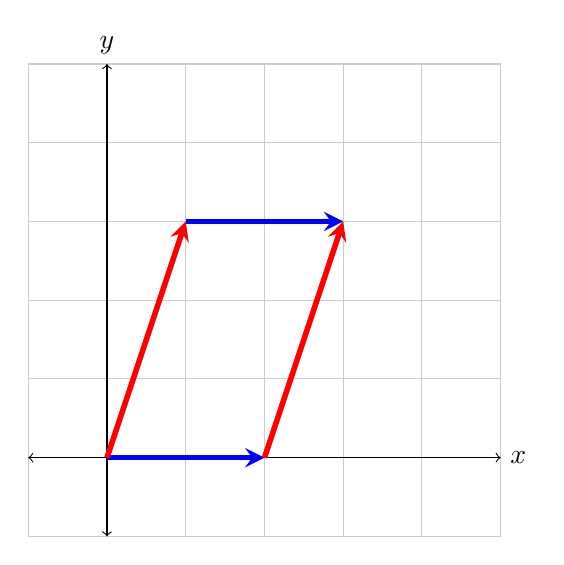
\begin{tikzpicture}
        \draw[thin,gray!40] (-1,-1) grid (5,5);
        \draw[<->] (-1,0)--(5,0) node[right]{$x$};
        \draw[<->] (0,-1)--(0,5) node[above]{$y$};
        \draw[line width=2pt,blue,-stealth](0,0)--(2,0) node[anchor=north] at (1,0){$\vecu$};
        \draw[line width=2pt, red, -stealth](0,0)--(1,3) node[anchor=east] at (.5,1.5){$\vecv$};
        \draw[line width=2pt,red,-stealth](2,0)--(3,3) node[anchor=east] at (.5,1){};
        \draw[line width=2pt, blue, -stealth](1,3)--(3,3) node[anchor=north] at (1,.5){};
        \end{tikzpicture}
        \end{center}
        The trick to finding the area here is to take move a triangle and fill in a gap. We do this like so:
        \begin{center}
        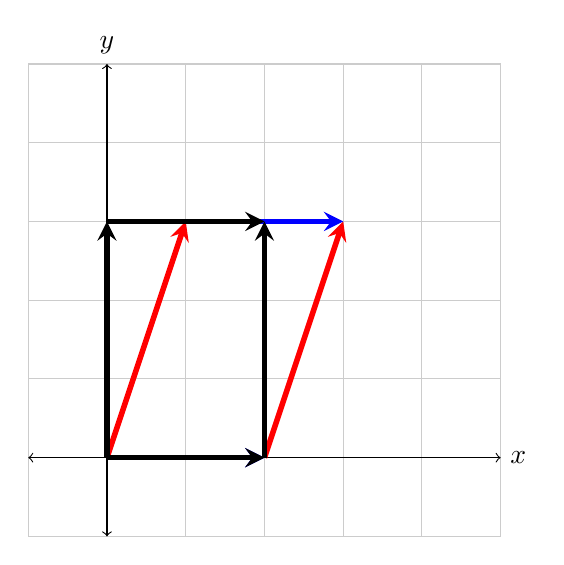
\begin{tikzpicture}
        \draw[thin,gray!40] (-1,-1) grid (5,5);
        \draw[<->] (-1,0)--(5,0) node[right]{$x$};
        \draw[<->] (0,-1)--(0,5) node[above]{$y$};
        \draw[line width=2pt,blue,-stealth](0,0)--(2,0) node[anchor=north] at (1,0){};
        \draw[line width=2pt, red, -stealth](0,0)--(1,3) node[anchor=east] at (.5,1.5){};
        \draw[line width=2pt,red,-stealth](2,0)--(3,3) node[anchor=east] at (.5,1){};
        \draw[line width=2pt, blue, -stealth](1,3)--(3,3) node[anchor=north] at (1,.5){};
        \draw[line width=2pt, black, -stealth](2,0)--(2,3) node[anchor=north] at (1,.5){};    
        \draw[line width=2pt, black, -stealth](0,0)--(0,3) node[anchor=north] at (1,.5){};
        \draw[line width=2pt, black, -stealth](0,0)--(2,0) node[anchor=north] at (1,.5){};
        \draw[line width=2pt, black, -stealth](0,3)--(2,3) node[anchor=north] at (1,.5){};
        \end{tikzpicture}
        \end{center}
        In the above, we've moved a triangle from the right, to the left, to make the black rectangle.  This rectangle then has an area of $2\cdot 3=6.$
        
        Let us see the way we can do this that does not require this extra work.  Let us place these vectors into a matrix:
        \[
        A=\begin{pmatrix} \vert & \vert \\ \vecu & \vecv \\ \vert & \vert \end{pmatrix}=
        \begin{pmatrix} 2 & 1\\ 0 & 3 \end{pmatrix}.
        \]
        Then $\det(A)$ will give us the area of this parallelogram! We have
        \[
        \det(A)=2\cdot 3 - 1\cdot 0 = 6.
        \]
        This begs the question, what is this formula in general? Note, that if you placed these vectors in $\R^3$ by adding a zero $z$-component, then 
        \[
        \|\vecu \times \vecv \| = 6,
        \]
        as well.
        \end{ex}
        
        In order to move to higher dimensions we must first settle the case in two dimensions.  So, to compute the \boldgreen{determinant} of a $2\times 2$-matrix
        \[
        [A]=\begin{pmatrix} a & b\\ c & d \end{pmatrix},
        \]
        we have
        \[
        \det([A]) = ad-bc.
        \]
        You can remember this by thinking that you multiply top left with bottom right, then subtract the product of top right with bottom left. Also, we will often use the notation of vertical bars around the matrix of numbers to denote a determinant. That is,
        \[
        \det([A]) = \left| \begin{matrix} a & b \\ c & d \end{matrix} \right|.
        \]
        
        Now, the generalization of a parallelogram to 3-dimensional space is called a \boldgreen{parralelepiped}.  Later on when we are doing calculus in 3-dimensional space it will become extremely important to be able to compute infinitesimal volumes (just like we have infinitesimal lengths $dx$) and they will be found via the volume of a parallelepiped.
        
        \begin{ex}{Volume of a Parallelepiped}{volume_of_parallelepiped}
        In $3$-dimensional space, we can take three vectors
        \[
        \vecu=\begin{pmatrix} 0 \\ 3 \\ 0 \end{pmatrix}\qquad
        \vecv=\begin{pmatrix} 1 \\ 0 \\ 0 \end{pmatrix}\qquad
        \vecw=\begin{pmatrix} 0 \\ 0 \\ 2 \end{pmatrix}.
        \]
        These, when combined properly, enclose a volume of a parallelepiped. 
\begin{center}
\tdplotsetmaincoords{60}{120} 
\begin{tikzpicture} [scale=3, tdplot_main_coords, axis/.style={->,black,thick}, 
vector/.style={-stealth,blue,very thick}, 
vector guide/.style={dashed,red,thick}]

%standard tikz coordinate definition using x, y, z coords
\coordinate (O) at (0,0,0);

%tikz-3dplot coordinate definition using x, y, z coords

\pgfmathsetmacro{\ax}{0.6}
\pgfmathsetmacro{\ay}{1}
\pgfmathsetmacro{\az}{0.8}

\coordinate (P) at (\ax,\ay,\az);

%draw axes
\draw[axis] (0,0,0) -- (1,0,0) node[anchor=north east]{$x$};
\draw[axis] (0,0,0) -- (0,1,0) node[anchor=north west]{$y$};
\draw[axis] (0,0,0) -- (0,0,1) node[anchor=south]{$z$};


\draw[line width=2pt, red, -stealth](0,0,0)--(0,3/4,0) node[anchor=north west] at (0,3/4,0){$\vecu$};
\draw[line width=2pt, blue, -stealth](0,0,0)--(1/4,0,0) node[anchor=north] at (1/4,0,0){$\vecv$};
\draw[line width=2pt, green, -stealth](0,0,0)--(0,0,1/2) node[anchor=east] at (0,0,1/2){$\vecw$};

\end{tikzpicture}
\end{center}
\begin{center}
\tdplotsetmaincoords{60}{120} 
\begin{tikzpicture} [scale=3, tdplot_main_coords, axis/.style={->,black,thick}, 
vector/.style={-stealth,blue,very thick}, 
vector guide/.style={dashed,red,thick}]

%standard tikz coordinate definition using x, y, z coords
\coordinate (O) at (0,0,0);

%tikz-3dplot coordinate definition using x, y, z coords

\pgfmathsetmacro{\ax}{0.6}
\pgfmathsetmacro{\ay}{1}
\pgfmathsetmacro{\az}{0.8}

\coordinate (P) at (\ax,\ay,\az);

%draw axes
\draw[axis] (0,0,0) -- (1,0,0) node[anchor=north east]{$x$};
\draw[axis] (0,0,0) -- (0,1,0) node[anchor=north west]{$y$};
\draw[axis] (0,0,0) -- (0,0,1) node[anchor=south]{$z$};


\draw[line width=2pt, red, -stealth](0,0,0)--(0,3/4,0) node[anchor=north west] at (0,1,0){};
\draw[line width=2pt, blue, -stealth](0,0,0)--(1/3,0,0) node[anchor=north] at (1/3,0,0){};
\draw[line width=2pt, green, -stealth](0,0,0)--(0,0,1/2) node[anchor=east] at (0,0,2/3){};

\draw[line width=2pt, red, -stealth](1/4,0,0)--(1/4,3/4,0) node[anchor=north west] at (1/3,2/3,3/3){};
\draw[line width=2pt, blue, -stealth](0,3/4,0)--(1/4,3/4,0) node[anchor=north] at (1/3,0,0){};
\draw[line width=2pt, green, -stealth](1/4,0,0)--(1/4,0,1/2) node[anchor=east] at (0,0,2/3){};

\draw[line width=2pt, red, -stealth](1/4,0,1/2)--(1/4,3/4,1/2) node[anchor=north west] at (1/3,2/3,3/3){};
\draw[line width=2pt, blue, -stealth](0,0,1/2)--(1/4,0,1/2) node[anchor=north] at (1/3,0,0){};
\draw[line width=2pt, green, -stealth](0,3/4,0)--(0,3/4,1/2) node[anchor=east] at (0,0,2/3){};

\draw[line width=2pt, red, -stealth](0,0,1/2)--(0,3/4,1/2) node[anchor=north west] at (1/3,2/3,3/3){};
\draw[line width=2pt, blue, -stealth](0,3/4,1/2)--(1/4,3/4,1/2) node[anchor=north] at (1/3,0,0){};
\draw[line width=2pt, green, -stealth](1/4,3/4,0)--(1/4,3/4,1/2) node[anchor=east] at (0,0,2/3){};
\end{tikzpicture}
\end{center}
Of course, I picked an easy example for the illustration.  But what is the volume? Here we again know we can compute this the usual way and we get that the volume is $1\cdot 1 \cdot 2 = 2.$ If we instead created a more complicated paralleliped like: 
\begin{figure}[H]
  \centering
  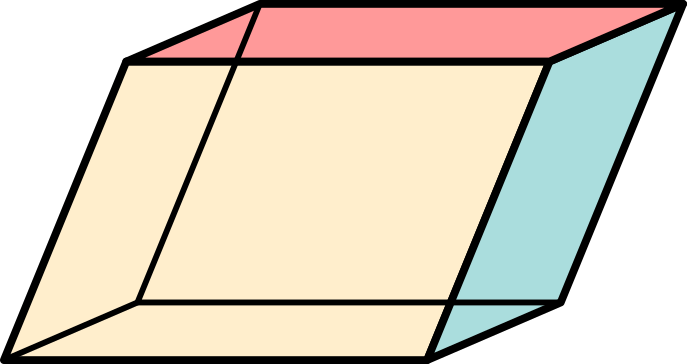
\includegraphics[width=.4\textwidth]{Figures_Part_4/Parallelepiped.png}
  \label{fig:paralellepiped}
\end{figure}
we must perform the same type of process as we did in Example \ref{ex:area_parallelogram}. The determinant is designed to do this process for us.
\end{ex}

Now, let us consider computing the determinant for a $3\times 3$-matrix $[A]$.  We should think of this matrix as being created from three vectors $\colA_1$, $\colA_2$, and $\colA_3$ as columns. So we have
\[
[A]=\begin{pmatrix} a_{11} & a_{12} & a_{13} \\ a_{21} & a_{22} & a_{23} \\ a_{31} & a_{32} & a_{33}  \end{pmatrix} =
\begin{pmatrix} \vert & \vert & \vert \\ \colA_1 & \colA_2 & \colA_3 \\ \vert & \vert & \vert \end{pmatrix},
\]
we want $\det(A)$ to reflect the the volume of a parallelepiped generated by $\colA_1$, $\colA_2$, and $\colA_3$. It turns out the way we compute $\det(A)$ comes from using the determinant of $2\times 2$-matrices.  Let me explain further.

Let me write this matrix as a tool:
\[
\begin{pmatrix} + & - & +\\ - & + & - \\ + & - & + \end{pmatrix}.
\]
What we will use this for is a memory tool when we do something called the \boldgreen{cofactor expansion}.  What I will do is choose a row or column to expand along.  For this example, let's choose the top row to expand along.  If we use this above matrix with pluses and minuses, we note that the top row will have signs $+-+$. These signs show up in our computation. We will also have to take into account the element in the original matrix and multiply by that.

We start with the top left of $[A]$ and we will have a $+$ sign.  The top left of $[A]$ is element $a_{11}$ and so we remove the first row and first column from $[A]$ to give the \boldgreen{cofactor matrix}
\[
\textrm{Cof}_{11}[A]=\begin{pmatrix} a_{22} & a_{23} \\ a_{32} & a_{33} \end{pmatrix}.
\]
Since ths is a $2\times2$-matrix, we can compute the determinant by \[
\det(\textrm{Cof}_{11})[A])=a_{22} a_{33}- a_{23} a_{32}.
\]
Then we continue expanding along this row and move on to the top middle of $[A]$ and will have a $-$ sign. The top middle element is $a_{12}$ and so we remove the first row and second column of $[A]$ to get
\[
\textrm{Cof}_{12}[A]=\begin{pmatrix} a_{21} & a_{23} \\ a_{31} & a_{33}\end{pmatrix}.
\]
Then we have that 
\[
\det(\textrm{Cof}_{12}[A])=a_{21}a_{33}-a_{31}a_{13}.
\]
Lastly, we move on to the top right of $[A]$ and will have a $+$ sign. The top right element is $a_{13}$ and so we remove the first row and third column of $[A]$ to give
\[
\textrm{Cof}_{13}[A]=\begin{pmatrix} a_{21} & a_{22} \\ a_{31} & a_{32} \end{pmatrix}.
\]
Then we have that
\[
\det(\textrm{Cof}_{13}[A])=a_{21}a_{32} - a_{22}a_{31}.
\]
We then define the determinant of $[A]$ to be
\[
\det([A]) = +a_{11} \det(\textrm{Cof}_{11}[A]) - a_{12} \det(\textrm{Cof}_{12}[A]) + a_{13} \det(\textrm{Cof}_{13}[A]).
\]
Similarly, if we expanded along the second column, for example, we would have that
\[
\det([A]) = -a_{12} \det(\textrm{Cof}_{12}[A]) + a_{22} \det(\textrm{Cof}_{22}[A]) - a_{32} \det(\textrm{Cof}_{32}[A]).
\]

\begin{ex}{Volume of a Parallelepiped from the Determinant}{vol_paralellepiped_from_det}
 Consider the vectors from the previous example
 \[
 \vecu = \begin{pmatrix} 0 \\ 3 \\ 0 \end{pmatrix} \qquad \vecv = \begin{pmatrix} 1 \\ 0 \\ 0 \end{pmatrix} \qquad \vecw = \begin{pmatrix} 0 \\ 0 \\ 2 \end{pmatrix}.
 \]
 Then we can place these three vectors into a matrix $[A]$ by
 \[
 [A]=\begin{pmatrix} \vert & \vert & \vert \\ \vecu & \vecv & \vecw \\ \vert & \vert & \vert \end{pmatrix} = \begin{pmatrix} 0 & 1 & 0 \\ 3 & 0 & 0 \\ 0 & 0 & 2 \end{pmatrix}.
 \]
 Then we can compute the determinant of $[A]$ by expanding along any row or column.  Typically, one wants to expand along a row or column with the most zeros. This will reduce the amount of work.  Here, it does not matter, so let us expand across the top row. We get
 \begin{align*}
 \det([A]) &= a_{11} \det(\textrm{Cof}_{11}[A]) - a_{12} \det(\textrm{Cof}_{12}[A]) + a_{13} \det(\textrm{Cof}_{13}[A])\\
 &=0\cdot \left| \begin{matrix} 0 & 0 \\ 0 & 2 \end{matrix} \right| - 1 \cdot \left| \begin{matrix} 3 & 0 \\ 0 & 2 \end{matrix} \right| + 0 \cdot \left| \begin{matrix} 3 & 0 \\ 0 & 0 \end{matrix} \right|\\
 &= -1 \cdot(3\cdot 2)\\
 &= -6.
 \end{align*}
 This determinant gave us exactly the negative of the volume of the parallelepiped. 
\end{ex}

From the previous example we saw that the determinant need not always be positive.  So we must say that the determinant of a matrix $[A]$ provides us the \boldgreen{signed volume} of the paralellepiped generated by its column vectors. The orientation is much like the orientation we saw for the cross product.


        \begin{exercise} Let
        \[
        A=\begin{pmatrix} 1 & 2 & 3 \\ 4 & 5 & 6 \\ 7 & 8 & 9 \end{pmatrix}.
        \]
        \begin{enumerate}[(a)]
            \item Find $\textrm{Cof}_{11}(A)$.
            \item Find $\textrm{Cof}_{22}(A)$.
            \item Find $\textrm{Cof}_{23}(A)$.
            \item Compute $\det(A)$.
        \end{enumerate}
        
        \end{exercise}
        
        \begin{question}
        What does it mean if $\det(A)=0$ for some matrix $A$?
        \end{question}
        
        \begin{answer}
        It means that we have a parallelopiped with zero volume.  Which means our three vectors actually lie in a plane, or even on a single line.  This is an important fact that will come up when we solve systems of equations!
        \end{answer}
        
        \begin{remark}
        Determinants can be computed in arbitrary dimension using the same process above. But, this will not be a worry for us at the moment.
        \end{remark}
        
        \subsection{Determinants and Systems of Equations}
    
    In defining the determinant, we found it useful for computing the volume of a parallelepiped. However, it does not stop there. If we adopt the convention that systems of linear equations such as
    \[
    [A]\vecx = \vecy
    \]
    where $[A]$ is a square matrix, then this is related to the question of whether the columns of $[A]$ form a spanning list of vectors for the vector space. 
    
    Since the determinant $\det([A])$ tells us the volume of the paralellepiped of the three column vectors creating $[A]$, if the volume is zero, then we know that the columns of $[A]$ must be linearly dependent. Since, if they were nonzero, the vectors would generate some volume.  Thus we have the following two propositions.
    
    \begin{prop}{Solutions to Homogeneous Equations}{solutions_to_homo}
        Consider the homogeneous equation
        \[
        [A]\vecx = \zerovec.
        \]
        Then we have the solutions:
        \begin{itemize}
            \item (Trivial) The only solution for $\vecx$ is $\vecx=\zerovec$ if and only if $\det(A)\neq 0$;
            \item There are multiple nonzero solutions for $\vecx$ if and only if $\det(A)= 0$.
        \end{itemize}
        \end{prop}
        
        The other way of wording the above proposition is that a matrix $[A]$ with a nonzero determinant equal has a nullspace that is trivial. In other words, if 
        \[
        \det([A])= 0
        \]
        then $\Null([A])=\{\zerovec\}$.  Otherwise, if the determinant is zero, then $\Null([A])$ contains more than just the zero vector. 
        
        There is a similar result for the inhomogeneous equations as well.  However, be careful to note the differences here. Afterwards we can discuss geometrically what is happening.
        
        \begin{prop}{Solutions to Inhomogeneous Equations}{solutions_to_inhomo}
        The inhomogenous equation
        \[
        [A]\vecx = \vecy
        \]
        (with $\vecy\neq \zerovec)$ have the following solutions:
        \begin{itemize}
            \item A unique solution for $\vecx$ if and only if $\det(A)\neq 0$;
            \item None or possibly infinitely many solutions for $\vecx$ if $\det(A)=0$.
        \end{itemize}
        \end{prop}
        
    \begin{exercise}
        Take the determinant and then attempt to solve the following homogeneous equations.
        \begin{enumerate}[(a)]
            \item Let 
            \[
            [A]=\begin{pmatrix}
            1 & 1 & 0\\
            1 & 0 & 5\\
            0 & 1 & 2
            \end{pmatrix}
            \]
            and solve $A\vecx=\zerovec.$
            \item Let
            \[
            [B]=\begin{pmatrix}
            2 & 3 & 1\\
            1 & 4 & 3\\
            1 & 2 & 1
            \end{pmatrix}
            \]
            and solve $[B]\vecx=\vecy.$
        \end{enumerate}
        \end{exercise}
        
        When thinking about these propositions, one should consider the case for functions $f\colon \R\to \R$.  In this case, we may have been handed a function $f$, a $y$ (output) value, and were asked to find what input $x$ corresponds to that $y$ value. That is, we want
        \[
        f(x)=y.
        \]
        Here we could sometimes find an inverse function $f^{-1}$ that would satisfy
        \[
        f^{-1}(y)=x.
        \]
        However, for example, if we had the function $f(x)=x^2$, then there was no inverse function.  Why? Well, say we let $y=1$, then $x=\pm 1$ are both solutions. This is not a valid function (since it does not pass the vertical line test). Also, if we provide $y=-1$, then there is no input value to achieve that output.
        
        We can also think of solving systems of linear equations in a geometrical way.  Let us consider two examples.  First, for the homogeneous case, we can take the homogeneous equation
        \[
        \begin{pmatrix} 1 & 0 & 0 \\ 0 & 1 & 0 \\ 0 & 0 & 0 \end{pmatrix} \begin{pmatrix} x \\ y \\ z \end{pmatrix} = \begin{pmatrix} 0 \\ 0 \\ 0 \end{pmatrix}.
        \]
        Here we can see that this gives the equations
        \[
        x=1,\qquad y=1,\qquad z=t.
        \]
        That is, $z$ is a free variable.  Hence here we find that the nullspace for the matrix 
        \[
        [A]=\begin{pmatrix} 1 & 0 & 0 \\ 0 & 1 & 0 \\ 0 & 0 & 0 \end{pmatrix}
        \]
        is given by
        \[
        \Null([A])=\Span\left( \begin{pmatrix} 0 \\ 0 \\ 1 \end{pmatrix}\right),
        \]
        which is the $z$-axis. If we think of columns of $[A]$ as vectors, then we find that the span of the columns is the $xy$-plane.  Thus, any $z$-component of an input vector does not affect the output.
        
        If we take this same matrix at consider an inhomogeneous problem, then the following equation has no solution
        \[
        \begin{pmatrix} 1 & 0 & 0 \\ 0 & 1 & 0 \\ 0 & 0 & 0 \end{pmatrix} \begin{pmatrix} x \\ y \\ z \end{pmatrix} = \begin{pmatrix} 0 \\ 0 \\ 1 \end{pmatrix}.        
        \]
        Why is that? Well, this gives rise to the equations
        \[
        x=1,\qquad y=1, \qquad 0\cdot z = 1,
        \]
        which has no solution for $z$.  This is exactly because of the fact that the columns of $[A]$ only span the $xy$-plane.  Taking a linear combination of the columns cannot give a resulting vector with a $z$-component.  We can visualize this as follows.  Let
        \[
        [T]=\begin{pmatrix} 1 & 0 & 0 \\ 0 & 1 & 0 \\ 0 & 0 & 0 \end{pmatrix} \qquad \textrm{and} \qquad \vecv = \begin{pmatrix} x \\ y \\ z \end{pmatrix},
        \]
        and we can see geometrically what this transformation does to a vector.  In a sense, this transformation removes a whole dimension from $\R^3$. It takes any $z$-component and removes it, hence we see that the transformation really takes the shadow of the input vector on the $xy$-plane.
        \begin{figure}[H]
            \centering
            \resizebox{.75\textwidth}{!}{\input{Figures_Part_4/linear_transform_kernel.pdf_tex}}
            %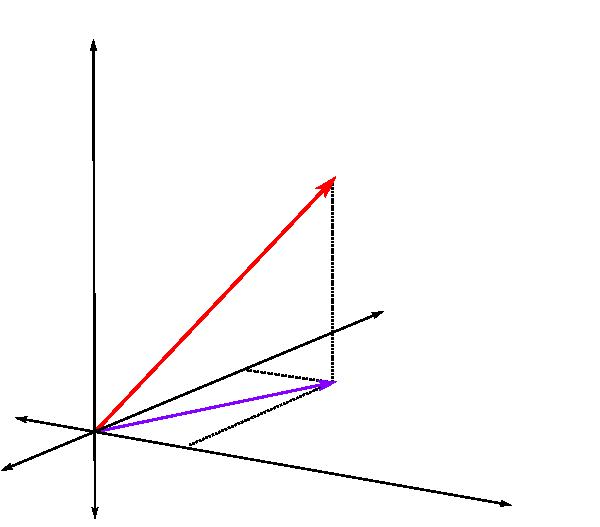
\includegraphics[width=.7\textwidth]{Figures_Part_4/linear_transform_kernel.pdf_tex}
        \end{figure}
        That is, we visually see that
        \[
        [T]\vecv = \begin{pmatrix} x \\ y \\ 0 \end{pmatrix}.
        \]
        
        Though this was a special circumstance, this is the exact picture to have in mind when solving systems of linear equations.  If we are given a point $\vecy$, a matrix $[A]$, and are asked to find the input vector $\vecx$ that solves
        \[
        [A]\vecx = \vecy,
        \]
        we are being asked if $\vecy$ is in the span of the columns of $[A]$ and $\vecx$ describes the coefficients for this linear combination.  And as we have seen, the columns of $[A]$ may or may not span the necessary amount of space to be able to create the output vector $\vecy$.
        
        The cross product and the determinant are related in some ways.  Since the formula for a cross product is not easy to memorize, and applying the cross product to basis vectors is tedious, it suffices to remember how to compute determinants of $3\times 3$-matrices and stop there. It is possible to compute the cross product by using the proper determinant. 
        
        \begin{ex}{Cross product from the Determinant}{cross_prod_det}
        You can compute the cross product from the determinant.  (You should be warned: this is an abuse of notation and a somewhat weird coincidence.) Let us create choose two vectors $\mathbf{v}$ and $\mathbf{w}$. We place them in a matrix $[A]$ as follows:
        \[
        A=
        \begin{bmatrix}
        \xhat & \yhat & \zhat\\
        v_x & v_y & v_z\\
        w_x & w_y & w_z
        \end{bmatrix}.
        \]
        Then $\det([A])$ will give us the cross product $\mathbf{v}\times \mathbf{w}$.  Just know that you are briefly ignoring the fact that $\xhat$, $\yhat$, $\zhat$ are actually vectors when you compute this.  Treat them as numbers until you get your final result.
        \end{ex}
        
        
        \subsection{Properties of determinants}
        There are a few nice properties of determinants to keep in mind. 
        \begin{itemize}
            \item \textbf{Transposition:} If we exchange rows for columns in a matrix (that is, to take the \emph{transpose matrix}, then the value of the determinant is the same. Given
            \[
            [A]=\begin{pmatrix}
            a_{11} & a_{12} & a_{13}\\
            a_{21} & a_{22} & a_{23}\\
            a_{31} & a_{32} & a_{33}
            \end{pmatrix}
            \]
            we write the transpose matrix
            \[
            [A]^T=\begin{bmatrix}
            a_{11} & a_{21} & a_{31}\\
            a_{12} & a_{22} & a_{32}\\
            a_{13} & a_{23} & a_{33}
            \end{bmatrix}.
            \]
            So $a_{ij}\mapsto a_{ji}$. Then
            \[
            \det([A])=\det([A]^T).
            \]
            
            \item \textbf{Multiplication by constants:} If we multiply a row or column by a scalar, then the determinant is also multiplied by that scalar.  So we have
            \[
            [A]_\alpha=\begin{bmatrix}
            \alpha a_{11} & \alpha a_{12} & \alpha a_{13}\\
            a_{21} & a_{22} & a_{23}\\
            a_{31} & a_{32} & a_{33}
            \end{bmatrix}
            \]
            Then
            \[
            \det([A]_\alpha)=\alpha \det([A]).
            \]
            And this holds no matter what row or column we scale.
            
            \item \textbf{Linear combinations of rows or columns:} If  we add a linear combination of columns (or rows) to any column (or row), then the determinant does not change. That is, if we have
            \[
            [A] = \begin{pmatrix} \vert & \vert & \vert \\ \colA_1 & \colA_2 & \colA_3 \\ \vert & \vert & \vert \end{pmatrix},
            \]
            then
            \[
            det([A]) = \left| \begin{matrix} \vert & \vert & \vert \\ \colA_1+\alpha\colA_2+\beta\colA_2 & \colA_2 & \colA_3 \\ \vert & \vert & \vert \end{matrix}\right|.
            \]
            Here we just showed adding a linear combination of two columns to the first column, but this holds in general for adding linear combinations of any columns to other columns or adding linear combinations of rows to any row.
            \item \textbf{Exchanging rows or columns:} If we swap rows or columns, the determinant is multiplied by $-1$. So we have
            \[
            \left|\begin{array}{ccc}
                a_{11} & a_{12} & a_{13} \\
                a_{21} & a_{22} & a_{23} \\
                a_{31} & a_{32} & a_{33}
            \end{array}\right|=-
            \left|\begin{array}{ccc}
                a_{12} & a_{11} & a_{13} \\
                a_{22} & a_{21} & a_{23} \\
                a_{32} & a_{31} & a_{33}
            \end{array}\right|
            \]
            Again, this holds for swapping any two rows (or any two columns).
            
            \item \textbf{Linearly-dependent rows or columns:} If a column (resp. row) of a matrix can be written as a linear combination of the other two columns (resp. rows), then the determinant is zero.  This is basically saying that all three vectors lie in a single plane and so the volume of the parallelepiped given by the three vectors (as columns in the matrix) create no volume.
            
            Say we can write
            \[
            \colA_1 = \alpha \colA_2 + \beta \colA_3
            \]
            Then $\det(A)=0.$ That is, if one column (or row) is in the span of the other columns (or rows), then the determinant of the matrix will be zero.
        \end{itemize}
        
        Another nice property of the determinant comes from the product of two matrices.  If we consider two square $n\times n$-matrices $[A]$ and $[B]$, then we can multiply both $[A]$ and $[B]$. Then we have that the determinant is \boldgreen{multiplicative} in that
        \[
        \det([A][B])=\det([A])\det([B]).
        \]
        This turns out to be a very useful property of the determinant.  If one thinks of the determinant as describing how much the basis vectors $\xhat$, $\yhat$, and $\zhat$ are stretched by the composition transformation $[A][B]$, then this is saying that the product transformation stretches the vectors by first stretching by $[A]$ then by $[B]$.
        
        \subsection{The Trace}
        
        The determinant was an example of an \boldgreen{invariant} of a matrix $[A]$. That is, it is a quantity that does not change even when certain operations are performed. These operations that leave the determinant invariant were the row operations.
        
        Given a square matrix $[A]$, we can associate to it another invariant called the \boldgreen{trace} which is rather easy to compute.  The trace of a matrix is simply the sum of the diagonal entries. That is, given
        \[
        [A]=\begin{pmatrix} a_{11} & a_{12} & a_{13} \\ a_{21} & a_{22} & a_{23} \\ a_{31} & a_{32} & a_{33} \end{pmatrix}
        \]
        then the trace of $[A]$ is
        \[
        \tr([A]) = a_{11}+a_{22}+a_{33} = \sum_{i=1}^3 a_{ii}.
        \]
        
        \begin{ex}{Trace of a Matrix}{trace_of_matrix}
        Consider the matrix
        \[
        [A]=\begin{pmatrix} 1 & 2 & 3 \\ 4 & 5 & 6 \\ 7 & 8 & 9 \end{pmatrix}.
        \]
        Then we have
        \[
        \tr([A])=1 + 5 + 9 = 15.
        \]
        \end{ex}
        
        The trace has a few nice properties as well. First, the trace is \boldgreen{additive} so that if we have two $n\times n$-matrices $[A]$ and $[B]$ then 
        \[
        \tr([A]+[B]) = \tr([A]+[B]).
        \]
        However, the trace is not multiplicative like the determinant!  
        
        But, if we have a product of matrices $[A]$, $[B]$, and $[C]$, then we have
        \[
        \tr([A][B][C])=\tr([B][C][A])=\tr([C][A][B]),
        \]
        which is a way of saying that we can \boldgreen{cyclically permute} products of matrices with the trace. For a product of two matrices this means
        \[
        \tr([A][B])=\tr([B][A]).
        \]
        
        Lastly, if we scale a matrix by a constant, then that scales the trace by a constant as well. That is,
        \[
        \tr(\alpha[A])=\alpha \tr([A]).
        \]
        
        The invariant actions for the trace are a require a bit more knowledge that we will develop in the next section.
        
    \section{Inverse Matrices and Similarity }
        As previously mentioned, we can be handed an equation such as
        \[
        f(x)=y,
        \]
        and attempt to find an inverse function $f^{-1}$ so that we have
        \[
        f^{-1}(y)=x.
        \]
        This is generally a very useful tactic to use.  In this case, we can quickly find an input $x$ for a given $y$ without having to solve a new set of equations each time.
        
        Since matrices are representations of linear functions, we can attempt to find an inverse for matrices as well.  If we are given the equation
        \[
        [A]\vecx=\vecy,
        \]
        then we can try to determine the matrix $[A]^{-1}$ so that
        \[
        \vecx = [A]^{-1}\vecy.
        \]
        Hence, if we are given any output vector $\vecy$, we can quickly find the corresponding input vector $\vecx$ through matrix multiplication. We call this special matrix $[A]^{-1}$ the \boldgreen{inverse matrix}\index{inverse!matrix}. In this case $[A]$ \underline{must} be square or else this is not at all possible! If a given matrix $[A]$ has an inverse matrix we say that $[A]$ is \boldgreen{invertible}\index{invertible}.
        
        Since $[A]$ is a function (specifically, a linear transformation), we do not always have an inverse. However, the determinant carries enough data to tell us when a matrix is invertible.  Suppose that $[A]$ is an $n\times n$-matrix, it turns out that $[A]^{-1}$ exists when the columns of $[A]$ span $\R^n$.  Based on our knowledge of the determinat, we can phrase this another way.
        
        \begin{prop}{Existence of Inverse}{existence_of_inverse}
        If $\det([A])\neq 0$, then $[A]^{-1}$ exists and is unique.
        \end{prop}
        
        When speaking of inverses, we must also realize what function acts as the \boldgreen{identity}\index{identity}.  For example, if we have a function $f(x)=y$ that is invertible. Then we know
        \[
        f(f^{-1}(y))=y \qquad \textrm{and} \qquad f^{-1}(f(x))=x.
        \]
        In other words, the composite functions
        \[
        f\circ f^{-1} \qquad \textrm{and} \qquad f^{-1} \circ f
        \]
        give the same output value as the given input value.  So, we must ask what matrix (or linear transformation) gives the same output value for a given input value.
        
        \begin{df}{Identity Matrix}{identity_matrix}
        We call the matrix $[I]$ with entries 
        \[[I]_{ij}=
        \begin{cases}
        1 \textrm{ if } i=j\\
        0 \textrm{ elsewise}
        \end{cases}
        \]
        the \boldgreen{identity matrix}\index{identity!matrix}.  For example, the $3\times 3$ identity matrix is
        \[[I]=
        \begin{bmatrix}
        1 & 0 & 0\\
        0 & 1 & 0\\
        0 & 0 & 1
        \end{bmatrix}.
        \]
        \end{df}
        
        Since we can multiply matrices and vectors, we should see how the identity matrix acts on each.  Just as we had with functions, the identity should fix the input value and thus give the same value as the output.  In other words, this is the matrix that ``does nothing."
        
        \begin{prop}{Identity Matrix Fixes Vectors}{identity_fixes_vectors}
        For any vector $\vecv$ we have that
        \[
        [I]\vecv=\vecv.
        \]
        In fact, for any equal sized square matrix $[A]$, we have that
        \[
        [I][A]=[A][I]=[A].
        \]
        \end{prop}
        
        \begin{exercise}
        Let
        \[
        \vecv=\begin{pmatrix} 1 \\ 2 \\ 3 \end{pmatrix}.
        \]
        Show that
        \[
        [I]\vecv=\vecv.
        \]
        
        Similarly, let
        \[
        [A]= \begin{bmatrix}
        1 & 2 & 3\\
        4 & 5 & 6\\
        7 & 8 & 9
        \end{bmatrix}.
        \]
        Show that
        \[
        [I][A]=[A].
        \]
        \end{exercise}
        
        The most important property of the inverse is that given an invertible matrix $[A]$ we have that
        \[
        [A]^{-1}[A]=[A][A]^{-1}=I.
        \]
        This is exactly like the inverse of a function (as it should be since $[A]$ is just a special type of function).  To think of this geometrically, we also know that if $[A]$ is an $n\times n$-matrix, the columns of $[A]$ must span $\R^n$.  If this were not the case, say with the matrix
        \[
        [A]=\begin{pmatrix} 1 & 0 & 0 \\ 0 & 1 & 0 \\ 0 & 0 & 0 \end{pmatrix},
        \]
        then we cannot invert the matrix.  See for example, this matrix above is the function that forgets the $z$-component of an input vector $\vecx$. So if we take
        \[
        \begin{pmatrix} 1 & 0 & 0 \\ 0 & 1 & 0 \\ 0 & 0 & 0 \end{pmatrix} \begin{pmatrix} x \\ y \\ z \end{pmatrix} = \begin{pmatrix} x \\ y \\ z \end{pmatrix},
        \]
        we see that we cannot possibly recover the $z$-input. Why? We could have given any value for the $z$-input, but the output is always zero which gives us no means of recovering the true input value.  By this argument, we can see that if a matrix $[A]$ has a nontrivial nullspace, we cannot invert it.  This is equivalent to the statement that $\det([A])$ must be nonzero in order to construct $[A]^{-1}$.
        
        \subsubsection{Inverting a matrix}
        
        Since we know a matrix can be inverted, we should also work on constructing the inverse. So, for example, let $[A]$ be a $3\times 3$ invertible matrix then we can create the augmented matrix
        \[
        [M]=
        \left( \begin{array}{ccc|ccc}
        a_{11} & a_{12} & a_{13} & 1 & 0 & 0 \\
        a_{21} & a_{22} & a_{23} & 0 & 1 & 0 \\
        a_{31} & a_{32} & a_{33} & 0 & 0 & 1 
        \end{array} \right),
        \]
        where we have augmented the identity matrix [I] along with the matrix [A]. From here, we can row reduce the left portion until we have
        \[
        \left( \begin{array}{ccc|ccc}
        1 & 0 & 0 & \tilde{a}_{11} & \tilde{a}_{12} & \tilde{a}_{13}\\
        0 & 1 & 0 & \tilde{a}_{21} & \tilde{a}_{22} & \tilde{a}_{23} \\
        0 & 0 & 1 & \tilde{a}_{31} & \tilde{a}_{32} & \tilde{a}_{33} 
        \end{array} \right),
        \]
        where $\tilde{a}_{ij}^{-1}$ is the entry of the matrix $A^{-1}$. 
        
        Note that in the $3\times 3$ case that we have
        \[
        [I] = \begin{pmatrix} \vert & \vert & \vert \\ \xhat & \yhat & \zhat \\ \vert & \vert & \vert \end{pmatrix}.
        \]
        Hence, the idea of the augmented matrix above is that we are checking that if $\xhat$, $\yhat$, or $\zhat$ are given as output vectors, then we can construct an input vector corresponding to those output values. 
        
        
        \begin{exercise}
        Let
        \[
        [A]=\begin{pmatrix}
        1 & 2\\
        2 & 1
        \end{pmatrix}.
        \]
        \begin{enumerate}[(a)]
            \item Find $[A]^{-1}$.
            \item Compute $\det([A])$ and $\det([A]^{-1})$. What do you notice about $\det([A]^{-1})$ compared to $\det([A])$?
        \end{enumerate}
        \end{exercise}
        
        \subsection{Properties Related to Inverse Matrices}
        Matrices that are invertible are rather special and with that comes some related properties. For example, we have that
        \[
        \det([I])=1.
        \]
        If we take that along with the fact that
        \[
        \det([A][B])=\det([A])\det([B]),
        \]
        then we have the following proposition.
        
        \begin{prop}{Determinant of Inverse Matrix}{det_of_inverse}
        We have that
        \[
        \det(A^{-1})=\frac{1}{\det(A)}.
        \]
        \end{prop}
        
        Also, the inverse of an inverse matrix is the original matrix.  That is, 
        \[
        \left([A]^{-1}\right)^{-1} = [A].
        \]
        
        Lastly, one may consider the inverse of a product of matrices.  If we have the product of two matrices
        \[
        [A][B],
        \]
        then to invert this product, we have to undo the transformations in the proper order. We refer to this as \emph{socks and shoes} since this is analogous to how we put on socks then shoes and take them off in the reverse order! Specifically, we have that
        \[
        ([A][B])^{-1}=[B]^{-1}[A]^{-1},
        \]
        which we can see is correct by
        \[
        ([A][B])^{-1}[A][B] = [B]^{-1}[A]^{-1}[A][B]^{-1} = [B]^{-1}[B]=[I].
        \]
        
        Invertible matrices are also matrices that can be used to simplify other matrices.  Typically, when we are handed a matrix $[A]$, we only care about the main invariant properties of that matrix. That is, properties which are captured through a certain type of operation.  
        
        \begin{df}{Similar Matrices}{similar_matrices}
        Let $[A]$ be an $n\times n$-square matrix, and $[P]$ an $n\times n$ invertible matrix. Then we say that the matrix $[Q]$ is \boldgreen{similar}\index{similar} to the matrix $[A]$ if we have
        \[
        [Q]=[P]^{-1}[A][P].
        \]
        \end{df}
        
        As it turns out that there is typically a ``nicest looking" matrix that is similar to a given matrix $[A]$.  This will be one of the main goals of the Eigenvalue problem which we will see in the next section.  The two main invariant quantities we associate to a matrix are the trace and determinant and thus, we should hope they remain invariant for any similar matrix. This motivates the following proposition which we shall prove.
        
        \begin{prop}{Trace and Determinant are Invariant}{trace_det_invariant}
            Let $[A]$ and $[Q]$ be similar matrices.  Then we have that
            \[
            \det([A])=\det([Q] \qquad \textrm{and} \qquad \tr([A])=\tr([Q]).
            \]
            \tcblower
            \begin{proof}
            Since $[A]$ and $[Q]$ are similar, there exists an invertible matrix $[P]$ so that
            \[
            [Q]=[P]^{-1}[A][P].
            \]
            Then we have that
            \begin{align*}
                \det([Q])&= \det([P]^{-1}[A][P])\\
                &= \det([P]^{-1})\det([A])\det([P])\\
                &=\frac{1}{\det([P])} \det([A])\det([P])\\
                &=\det([A]).
            \end{align*}
            Similarly for the trace we have,
            \begin{align*}
                \tr([Q])&= \tr([P]^{-1}[A][P])\\
                &= \tr([P][P]^{-1}[A])\\
                &= \tr([I][A])\\
                &=\tr([A]).
                \end{align*}
            \end{proof}
        \end{prop}
        
   \section{The Eigen-Problem}
   \index{eigen}
        Given a square matrix $[A]$, what is the ``nicest looking" matrix $[\Lambda]$ that is similar to $[A]$? This is a question of fundamental importance in many ways.  For one, it allows us to simplify down a linear transformation into the form that is the most easy to understand.  Also, the problem is very physical as it turns out to be exactly the description of Schr\"odinger's equation. All of this can be stated in the following way.
        
        \begin{question}
        Given a square matrix $[A]$, does there exist a scalar $\lambda$ and a corresponding vector $\evec$ such that
        \[
        [A]\evec=\lambda \evec?
        \]
        \end{question}
        
        This type of equation is called an \boldgreen{eigenvalue equation}.  We can immediately compare it to Schr\"odinger's equation which takes the form
        \[
        H(x)\Psi(x) = E\Psi(x)
        \]
        where $H(x)$ is the Hamiltonian, and $E$ is the energy value for the wavefunction $\Psi(x)$.  It turns out that this is an eigenvalue equation, but in this case $H(x)$ can be something other than a matrix of constant numbers (which makes it more complicated to solve).
        
        \begin{df}{Eigenvalues and Eigenvectors}{eigenvals_eigenvects}
        Let $[A]$ be a square matrix.  Then if we have a scalar $\lambda$ and $\evec$ satisfying
        \[
        [A]\evec=\lambda \evec
        \]
        we call $\lambda$ an \boldgreen{eigenvalue}\index{eigen!value} and $\evec$ the corresponding \boldgreen{eigenvector}\index{eigen!vector}.
        \end{df}
        
        \begin{remark}
            It's important to note that an eigenvalue \emph{corresponds} to an eigenvector.  They are insperable partners! 
        \end{remark}
        
        \begin{question}
        Why in the world should we care about this? What are the applications? 
        \end{question}
        
        \begin{answer}~
        \begin{itemize}
            \item First off, mathematically what this is saying is we can find vectors that are affected by a linear transformation (a matrix $[A]$) in the simplest possible way.  That is, the matrix just scales the vector!  If we are able to find a basis of eigenvectors, then we can understand how a matrix $[A]$ acts entirely by scaling certain directions. This last part is not always possible, but we are not concerned with this.
            \item The applications are extremely far ranging.  
            \begin{itemize}
                \item Data analysis: Understanding the structure of a data set.
                \item Mechanics: Understanding rotational motion.
                \item Quantum Mechanics: The whole theory of ``first quantization" is about solving the eigen-equation called \emph{Sch\"odinger's equation}. There, it turns out that eigenvectors are the observable states for a quantum system.
                \item Molecular Orbitals: Molecular orbitals are eigenvectors of the Fock operator.
                \item Differential Equations: We can often recast differential equations as eigen-problems which are, in general, fairly easy to solve in comparison. Here eigenvectors are functions.
                \item Finance: Breaking down portfolios based on risk and returns.
                \item Geology: The study of glacial till.
                \item Singular Value Decomposition and Principal Component Analysis: A generalization of the eigen-problem.
            \end{itemize}
        \end{itemize}
        \end{answer}
        
        Great, so now we are motivated.  But, how can we hope to find these eigenvalues and eigenvectors?  
        
        We begin with the equation
        \[
        [A]\evec=\lambda \evec
        \]
        and we subtract $\lambda \evec$ from both sides to yield
        \begin{align*}
            [A]\evec-\lambda \evec&=\zerovec.
        \end{align*}
        Remember that we can multiply by the identity matrix and not change a single thing.  We do this like so.
        \begin{align*}
            [A]\evec- I \lambda \evec&=\zerovec\\
            ([A]-\lambda [I])\evec&=\zerovec.
        \end{align*}
        This means we have reduced the problem to solving the homogeneous equations for a slightly different matrix $[A]-\lambda [I]$.  
        
        Recall that we had a proposition that said these homogeneous equations have nontrivial solutions if 
        \[
        \det([A]-\lambda [I])=0.
        \]
        This determinant condition gives us an equation that allows us to determine a value for $\lambda$. Specifically, this is a polynomial equation in the variable $\lambda$ that we refer to as the \boldgreen{characteristic polynomial}. Since this is a polynomial equation, we will always be able to find roots over the field of complex numbers.
        
        When we then know $\lambda$, we can solve for $\evec$ by plugging in the known $\lambda$ value and solving the homogeneous equations. Let me put this down in an algorithmic way as follows.
        \begin{enumerate}
            \item Let $\lambda$ be a variable.  Then we make the matrix $[A]-\lambda [I]$.
            \item Take the determinant of $[A]-\lambda [I]$ and set it equal to zero. That is,
            \[
            \det([A]-\lambda [I])=0.
            \]
            This will give you a polynomial equation with the variable $\lambda$.   
            \item You will find (possibly) multiple values of $\lambda$ from the determinant above.  
            \item For each $\lambda_i$, you will find an eigenvector $\evec_i$ by solving the homogeneous equation
            \[
            ([A]-\lambda_i [I])\evec_i=\zerovec.
            \]
            In other words, $\evec_i$ is in the nullspace  $\Null([A]-\lambda_i[I])$. 
        \end{enumerate}
        
        \begin{ex}{Eigenvalues of a Diagonal Matrix}{eigenvalues_of_diagonal}
        The easiest example of the eigenvalue problem is finding the eigenvectors and eigenvalues of a \emph{diagonal} matrix.  In this case, let
        \[
        [A]=\begin{pmatrix}
        1 & 0 & 0\\
        0 & 2 & 0\\
        0 & 0 & 3
        \end{pmatrix}.
        \]
        \begin{enumerate}
            \item Take $\lambda$ to be a variable and put
            \[
            A-\lambda I = \begin{bmatrix}
            1-\lambda & 0 & 0\\
            0 & 2-\lambda & 0\\
            0 & 0 & 3-\lambda
            \end{bmatrix}.
            \]
        \item Now we take the determinant of $[A]-\lambda [I]$
        \[
        \det([A]-\lambda [I])= (1-\lambda)(2-\lambda)(3-\lambda).
        \]
        We set this equal to zero
        \[
        (1-\lambda)(2-\lambda)(3-\lambda)=0.
        \]
        \item Note that this has solutions $\lambda_1=1$, $\lambda_2=2$, and $\lambda_3=3$.  
        \item 
        \begin{itemize}
            \item \textbf{$\lambda_1=1$:} We take
            \[
            ([A]-1[I])\evec_1=\zerovec.
            \]
            We solve this by making the augmented matrix:
            \[
            [M]=\left( \begin{array}{ccc|c}
                 1-1 & 0 & 0 & 0\\
                 0 & 2-1 & 0 & 0\\
                 0 & 0 & 3-1 & 0
            \end{array}\right).
            \]
            We can then perform the row reduction steps to get this augmented matrix to RREF.  In our case, this is essentially done and the system of equations reads:
            \begin{align*}
                0x+0y+0z&=0 ~\implies~ x=t\\
                0x+1y+0z&=0 ~\implies~ y=0\\
                0x+0y+2z&=0 ~\implies~ z=0.
            \end{align*}
            So we have a solution
            \[
            \evec_1 =\begin{bmatrix}
            t\\ 0\\ 0\\
            \end{bmatrix}.
            \]
            We usually prefer our eigenvectors to be normalized, so in this case we take $t=1$ and say that the eigenvector is 
            \[
            \evec_1 =\begin{pmatrix}
            1\\ 0 \\ 0
            \end{pmatrix}.
            \]
            \item \textbf{$\lambda_2=2$:} I'll suppress the work here but the eigenvector is
            \[
            \evec_2 = \begin{pmatrix}
            0 \\ 1 \\ 0
            \end{pmatrix}.
            \]
            \item \textbf{$\lambda_3=3$:} Again, the eigenvector is
            \[
            \evec_3=\begin{bmatrix}
            0 \\ 0 \\ 1
            \end{bmatrix}.
            \]
        \end{itemize}
        \end{enumerate}
        \end{ex}
        
        The above case is the easiest case for solving the eigenvalue problem, and it is also one of the reasons for the eigenvalue problem which we will see in the next section.  We can consider another example.
        
        \begin{ex}{A $2\times 2$ Eigen-problem}{2x2eigen}
         Consider the matrix
         \[
         [A]=\begin{pmatrix} 0 & 1 \\ 1 & 0 \end{pmatrix}.
         \]
         Now, we take
         \begin{align*}
             \det([A]-\lambda [I])&= \left| \begin{matrix} -\lambda & 1 \\ 1 & -\lambda \end{matrix} \right|\\
             &= \lambda^2-1.
         \end{align*}
         Hence, setting the determinant equal to zero we find that
         \[
         \lambda = \pm 1,
         \]
         and we put $\lambda_1=1$ and $\lambda_2=-1$.
         \begin{itemize}
             \item \textbf{$\lambda_1=1$:} We take
             \[
             ([A]-1[I])\evec_1 = \zerovec
             \]
             which gives us the augmented matrix
             \[
             [M] =\left( \begin{array}{cc|c} -1 & 1 & 0\\ 1 & -1 &0 \end{array}\right),
             \]
             which we can reduce to
             \[
             \left( \begin{array}{cc|c} -1 & 1 & 0\\ 0 & 0 & 0 \end{array}\right),
             \]
             which gives the equation 
             \[
             x=y,
             \]
             hence we can take $x=1$ which gives $y=1$ and hence
             \[
             \evec_1 = \begin{pmatrix} 1 \\ 1 \end{pmatrix}.
             \]
             \item \textbf{$\lambda_2=-1$:} We take
             \[
             ([A]+1[I])\evec_1 = \zerovec
             \]
             which gives us the augmented matrix
             \[
             [M] =\left( \begin{array}{cc|c} 1 & 1 & 0\\ 1 & 1 &0 \end{array}\right),
             \]
             which we can reduce to
             \[
             \left( \begin{array}{cc|c} 1 & 1 & 0\\ 0 & 0 & 0 \end{array}\right),
             \]
             which gives the equation 
             \[
             x=-y,
             \]
             hence we can take $x=1$ which gives $y=-1$ and hence
             \[
             \evec_2 = \begin{pmatrix} 1 \\ -1 \end{pmatrix}.
             \]
         \end{itemize}
         Thus we have our eigenvalue and eigenvector pairs
         \[
         \lambda_1 = 1 \qquad \evec_1 = \begin{pmatrix} 1 \\ -1 \end{pmatrix}
         \]
         and
         \[
         \lambda_2 = -1 \qquad \evec_2 = \begin{pmatrix} 1 \\ 1 \end{pmatrix}.
         \]
        \end{ex}
        
        Every eigenvalue problem will behave this same way, however, since we need to factor polynomial equations it is best to now consider vectors that have complex entries in them. That is, we can more easily work over the vector space $\C^n$ where vectors are given by
        \[
        \vecv = \begin{pmatrix} z_1 \\ z_2 \\ \vdots \\ z_n \end{pmatrix} \qquad \textrm{with each $z_i\in \C$}.
        \]
        Let us see why this is necessary with an example.
        
        \begin{ex}{A Complex $2\times 2$ Eigen-problem}{2x2eigen}
         Consider the matrix
         \[
         [A]=\begin{pmatrix} 0 & -1 \\ 1 & 0 \end{pmatrix},
         \]
         and take
         \begin{align*}
             \det([A]-\lambda [I])&= \left| \begin{matrix} -\lambda & -1 \\ 1 & -\lambda \end{matrix} \right|\\
             &= \lambda^2+1.
         \end{align*}
         Then after setting the determinant equal to zero we find that
         \[
         \lambda = \pm i.
         \]
         This tells us the eigenvalues for this matrix are complex! Hence the necessity for working with complex numbers as opposed to reals.
         
         Now, we put $\lambda_1=i$ and $\lambda_2=-i$.
         \begin{itemize}
             \item \textbf{$\lambda_1=i$:} We take
             \[
             ([A]-i[I])\evec_1 = \zerovec
             \]
             which gives us the augmented matrix
             \[
             [M] =\left( \begin{array}{cc|c} -i & -1 & 0\\ 1 & -i &0 \end{array}\right),
             \]
             which we can reduce to
             \[
             \left( \begin{array}{cc|c} i & 1 & 0\\ 0 & 0 & 0 \end{array}\right),
             \]
             which gives the equation 
             \[
             ix=-y,
             \]
             hence we can take $x=1$ which gives $y=-i$ and hence
             \[
             \evec_1 = \begin{pmatrix} 1 \\ -i \end{pmatrix}.
             \]
             \item \textbf{$\lambda_2=-1$:} We take
             \[
             ([A]+1[I])\evec_1 = \zerovec
             \]
             which gives us the augmented matrix
             \[
             [M] =\left( \begin{array}{cc|c} i & -1 & 0\\ 1 & i &0 \end{array}\right),
             \]
             which we can reduce to
             \[
             \left( \begin{array}{cc|c} -i & 1 & 0\\ 0 & 0 & 0 \end{array}\right),
             \]
             which gives the equation 
             \[
             ix=y,
             \]
             hence we can take $x=1$ which gives $y=i$ and hence
             \[
             \evec_2 = \begin{pmatrix} 1 \\ i \end{pmatrix}.
             \]
         \end{itemize}
         Thus we have our eigenvalue and eigenvector pairs
         \[
         \lambda_1 = i \qquad \evec_1 = \begin{pmatrix} 1 \\ -i \end{pmatrix}
         \]
         and
         \[
         \lambda_2 = -i \qquad \evec_2 = \begin{pmatrix} 1 \\ i \end{pmatrix}.
         \]
        \end{ex}
        
        Now, let us revisit something we have seen before and relate this to eigenvalues. First, we must realize that not all eigenvalues for a matrix will be unique.  Take for example,
        \[
        [I]=\begin{pmatrix} 1 & 0 & 0 \\ 0 & 1 & 0 \\ 0 & 0 & 1 \end{pmatrix}
        \]
        which has an eigenvalue of 1 repeated three times. We call the number of times an eigenvalue is repeated the \boldgreen{algebraic multiplicity}. 
        
        \begin{exercise}
        Verify this above statement.
        \end{exercise}
        
        \begin{thm}{Determinant, Trace, and Eigenvalues}{det_trace_eigenvalues}
            Let $[A]$ be an $n\times n$-matrix with eigenvalues $\lambda_1,\lambda_2,\dots,\lambda_k$ that occur $m_1,m_2,\dots,m_k$ times respectively (i.e., the algebraic multiplicity), then we have
            \[
            \det([A])=\lambda_1^{m_1} \lambda_2^{m_2} \cdots \lambda_k^{m_k}
            \]
            and
            \[
            \tr([A])=m_1 \lambda_1 + m_2 \lambda_2 + \cdots + \lambda_k m_k.
            \]
        \end{thm}
        
        The way we can think of this is that the eigenvalues tell us how different directions are stretched. The directions that are stretched are exactly the directions defined by the eigenvalues. Hence, it makes sense that the determinant is related to the eigenvalues. 
        
        \textcolor{red}{insert figure}
        
        \section{Diagonalization and Special Matrices}
            %diagonalization, diagonal matrices, hermititian matrices, blah blah
            The eigenvalue problem allows us to do a bit more with matrices.  We mentioned similar matrices previously, and one may wonder if given a matrix, if there is a similar matrix that is easier to understand.  The easiest matrices to understand are the \boldgreen{diagonal matrices} \index{matrix!diagonal} which take the form
            \[
            [\Lambda] = \begin{pmatrix} \lambda_1 & 0 & 0 & \cdots & 0 \\
                                        0 & \lambda_2 & 0 & \cdots & 0 \\
                                        0 & 0 & \ddots & \ddots & \vdots \\
                                        \vdots & \vdots & \ddots & \ddots & \vdots \\
                                        0 & 0 & 0 & \cdots & \lambda_n \end{pmatrix}
            \]
            To see why these matrices are nice, we can take an example of a $3\times 3$-matrix times an arbitrary 3-dimensional vector. So we have
            \[
            \begin{pmatrix} \lambda_1 & 0 & 0 \\ 0 & \lambda_2 & 0 \\ 0 & 0 & \lambda_3 \end{pmatrix} \begin{pmatrix} x \\ y \\ z \end{pmatrix}= \begin{pmatrix} \lambda_1 x \\ \lambda_2 y \\ \lambda_3 z \end{pmatrix}.
            \]
            As we can see, this matrix simply scales each of the inputs separately.  This gives us a transformation without rotation since it is only scaling.  No components are mixed together either.  
            
            It was exactly this that the eigenvalue problem went to solve.  Recall, we were given a matrix $[A]$ and were tasked with finding a eigenvector $\evec$ and corresponding eigenvalue $\lambda$ so that
            \[
            [A]\evec = \lambda \evec
            \]
            which says that the transformation $[A]$ simply scales the eigenvector $\evec$ by the eigenvalue $\lambda$.  Hence, if we are given a matrix $[A]$, we can find the eigenvalues and eigenvectors and construct a diagonal matrix!  Let us see how this shall work. 
            
            Consider for now the $3\times 3$-matrix case for $[A]$. Suppose that we find three eigenvalues $\lambda_1$, $\lambda_2$, and $\lambda_3$ that correspond to the eigenvectors $\evec_1$, $\evec_2$, and $\evec_3$ respectively.  Then we can construct the matrix
            \[
            [P]=\begin{pmatrix} \vert & \vert & \vert \\ \evec_1 & \evec_2 & \evec_3 \\ \vert & \vert & \vert \end{pmatrix}
            \]
            Now, in order for this matrix to be invertible we must have that the eigenvectors are linearly independent which we can verify by checking that $\det([P])\neq 0$. Then, when $[P]$ is invertible we can consider the following similar matrix
            \[
            [\Lambda] = [P]^{-1}[A][P].
            \]
            Let us see what happens when we consider multiplication by an arbitrary vector. We get
            \begin{align*}
                [P]^{-1}[A][P]\vecv &= [P]^{-1}[A]\begin{pmatrix} \vert & \vert & \vert \\ \evec_1 & \evec_2 & \evec_3 \\ \vert & \vert & \vert \end{pmatrix} \begin{pmatrix} x \\ y \\ z \end{pmatrix} \\
                &= [P]^{-1}[A](x\evec_1 + y \evec_2 + z\evec_3)\\
                &= [P]^{-1}\left( x [A]\evec_1 + y [A]\evec_2 + z [A]\evec_3 \right)\\
                &= [P]^{-1}( x \lambda_1 \evec_1 + y \lambda_2 \evec_2 + z \lambda_3 \evec_3).
            \end{align*}
            Now, we just need to know what the matrix $[P]^{-1}$ does.  To see what $[P]^{-1}$ does, we can just investigate $[P]$ acting on the unit basis vectors $\xhat$, $\yhat$, and $\zhat$.  We have that
            \[
            [P]\xhat = \evec_1 \qquad [P]\yhat = \evec_2 \qquad [P]\zhat =\evec_3
            \]
            and thus we have
            \[
            \xhat = [P]^{-1}\evec_1 \qquad \yhat = [P]^{-1} \evec_2 \qquad \zhat = [P]^{-1}\evec_3.
            \]
            Thus we have
            \[
            [P]^{-1}[A][P] \vecv = \lambda_1 x \xhat + \lambda_2 y \yhat J+ \lambda_3 z\zhat = \begin{pmatrix} \lambda_1 x \\ \lambda_2 y \\ \lambda_3 z \end{pmatrix}.
            \]
            Hence it must be that $[P]^{-1}[A][P]$ is a diagonal matrix! Specifically we have
            \[
            [\Lambda]=[P]^{-1}[A][P]
            \]
            where 
            \[
            [\Lambda] = \begin{pmatrix} \lambda_1 & 0 & 0 \\ 0 & \lambda_2 & 0 \\ 0 & 0 & \lambda_3 \end{pmatrix}.
            \]
            When a matrix $[A]$ is similar to a diagonal matrix $[\Lambda]$ we say that $[A]$ is \boldgreen{diagonalizable}.
            
            \subsection{Hermitian Matrices}
            Some types matrices have extra properties that make them worth studying on their own.  Specifically, when studying the physical world, we may want eigenvalues for a matrix to be real.  This isn't always, the case, but in quantum mechanics, for example, we will want energy eigenvalues to be real numbers.
            
            So begs the question as to what we need in order for a matrix to be guaranteed have real eigenvalues.  For now, we consider matrices with complex entries.  That is, take the matrix $[A]$ such that $a_{ij}\in \C$. Since real numbers are merely a subset of the complex numbers, everything done here works for the real case as well.  Given a matrix $[A]$, we define the  of $[A]$ \boldgreen{transpose} \index{matrix!transpose} to be the matrix $[A]^T$ whose entries are $a_{ji}$. That is, we swap rows with columns.  For example, we have
            \[
            [A] = \begin{pmatrix} a_{11} & a_{12} & a_{13} \\ a_{21} & a_{22} & a_{23} \\ a_{31} & a_{32} & a_{33} \end{pmatrix} \qquad \implies \qquad [A]^T = \begin{pmatrix} a_{11} & a_{21} & a_{31} \\ a_{12} & a_{22} & a_{32} \\ a_{13} & a_{23} & a_{33} \end{pmatrix} 
            \]
            If we have that
            \[
            [A]=[A]^T
            \]
            we say that $[A]$ is \boldgreen{symmetric}\index{matrix!symmetric}. Related to the transpose is the notion of the \boldgreen{adjoint of $[A]$} which we denote by $[A]^\dagger$.  The entries in $[A]^\dagger$ are given by $a_{ji}^*$ which means we take the transpose of $[A]$ and then complex conjugate the entries. That is, we have
            \[
                [A] = \begin{pmatrix} a_{11} & a_{12} & a_{13} \\ a_{21} & a_{22} & a_{23} \\ a_{31} & a_{32} & a_{33} \end{pmatrix} \qquad \implies \qquad [A]^\dagger = \begin{pmatrix} a_{11}^* & a_{21}^* & a_{31}^* \\ a_{12}^* & a_{22}^* & a_{32}^* \\ a_{13}^* & a_{23}^* & a_{33}^* \end{pmatrix}
            \]
            When a matrix $[A]$ is equal to its adjoint $[A]^\dagger$ we say that $[A]$ is \boldgreen{Hermitian}.  Hermitian and symmetric matrices play an important role in quantum mechanics due to the following theorem.  
            
            \begin{thm}{Hermitian Matrices Have Real Eigenvalues}{hermitian_real_eigen}
                Let $[A]$ be an $n\times n$-matrix with complex entries. We have that $[A]$ is Hermitian if and only if $[A]$ is diagonalizable and has only real eigenvalues.
            \end{thm}
            
            In fact, this is not the only result that is important.  There is something special about the eigenvectors for Hermitian matrices as well. But first we need a new definition.
            
            \begin{df}{Inner Product for Complex Vectors}{hermitian_inner_product}
                Let $\vecu,\vecv \in \C^n$ be $n$-dimensional vectors with complex entries. We define the \boldgreen{Hermitian inner product} of $\vecu$ and $\vecv$ to be
                \[
                \langle \vecu,\vecv \rangle \coloneqq \sum_{i=1}^n u_i v_i^*,
                \]
                where $v_i^*$ is the complex conjugate of the component $v_i$.
            \end{df}
            
            Take for example the vectors $\vecu,\vecv \in \C^2$ given by
            \[
            \vecu = \begin{pmatrix} 2i \\ 1+i \end{pmatrix} \qquad \textrm{and} \qquad \vecv = \begin{pmatrix} 1-i \\ 3 \end{pmatrix}.
            \]
            Then we can compute
            \begin{align*}
            \langle \vecu, \vecv \rangle &= \sum_{i=1}^2 u_i v_i^*\\
            &= (2i)(1-i)^* + (1ii)(3)^*\\
            &= (2i)(1+i)+(1+i)(3)\\
            &= 2i - 2 + 3 + 3i\\
            &=5i +1.
            \end{align*}
            
            \begin{remark}
                In the case where vectors are real, the Hermitian inner product is equivalent to the standard inner product (i.e., the dot product). Also, when a matrix has real entries, then $[A]^T=[A]^\dagger$ and so a real symmetric matrix is also Hermitian.
            \end{remark}
            
            \begin{thm}{Orthogonal Eigenvectors for Different Eigenvalues}{eigenvec_orthog}
                Let $[A]$ be Hermitian an $n\times n$-matrix with complex entries.  Then let $\evec_i$ and $\evec_j$ be eigenvectors corresponding to eigenvalues $\lambda_i$ and $\lambda_j$ such that $\lambda_i \neq \lambda_j$. Then we have that $\evec_i$ and $\evec_j$ are orthogonal (i.e., $\langle \evec_i, \evec_j\rangle=0$).
            \end{thm}
            
            Both of these theorems turn out to be exactly the conditions needed to properly build a quantum theory. Hence, studying Hermitian matrices is an important task all on its own.  
            
            \begin{ex}{Hermitian Matrix}{hermitian_matrix_ex}
                Consider the matrix
                \[
                [A]=\begin{pmatrix} 0 & -i \\ i & 0 \end{pmatrix}.
                \]
                Then we can show that $[A]$ is diagonalizable with real eigenvalues and orthogonal eigenvectors.  
                
                So we can find the characteristic polynomial by
                \[
                \det([A]-\lambda [I])=\lambda^2 - 1.
                \]
                Hence we set this equal to zero and find that we get the two real eigenvalues $\lambda_1=1$ and $\lambda_2=-1$.  Then we can find the eigenvector $\evec_1$ by solving
                \[
                ([A]-\lambda_1 [I])\evec_1 = 0.
                \]
                Specifically, we have the augmented matrix
                \[
                [M] = \left( \begin{array}{cc|c}
                    -1 & -i & 0 \\
                    i & -1 & 0
                \end{array}\right)
                \]
                Which we find gives a solution for the eigenvector 
                \[
                \evec_1 = \begin{pmatrix} -i \\ 1\end{pmatrix}.
                \]
                Similarly, we can get that the eigenvector corresponding to $\lambda_2=-1$ is given by 
                \[
                \evec_2=\begin{pmatrix} i \\ 1 \end{pmatrix}.
                \]
                Then, we can see that these eigenvectors are orthogonal by taking
                \[
                \langle \evec_1,\evec_2 \rangle = (-i)(i)^* + 1 = -1+1 = 0.
                \]
                Now, letting
                \[
                [P]=\begin{pmatrix} \vert & \vert \\ \evec_1 & \evec_2 \\ \vert & \vert \end{pmatrix} = \begin{pmatrix} -i & i \\ 1 & 1 \end{pmatrix}, 
                \]
                we can compute and find
                \[
                [P]^{-1} = \begin{pmatrix}
                \frac{i}{2} & \frac{1}{2} \\ \frac{-i}{2} & \frac{1}{2} \end{pmatrix}
                \]
                Then we can compute
                \begin{align*}
                    [P]^{-1}[A][P]&=\begin{pmatrix}
                \frac{i}{2} & \frac{1}{2} \\ \frac{-i}{2} & \frac{1}{2} \end{pmatrix} \begin{pmatrix} 0 & -i \\ i & 0 \end{pmatrix} \begin{pmatrix} -i & i \\ 1 & 1 \end{pmatrix}\\
                &= \begin{pmatrix} 1 & 0 \\ 0 & -1 \end{pmatrix}\\
                &= \begin{pmatrix} \lambda_1 & 0 \\ 0 & \lambda_2 \end{pmatrix}\\
                &= [\Lambda].
                \end{align*}
            \end{ex}
            
            Let us briefly revisit the particle in the 1-dimensional box.  There, we found states of the system were given by
            \[
            \psi_n(x) = \sqrt{\frac{2}{L}} \sin\left(\frac{n\pi x}{L}\right).
            \]
            We stated that the states were orthogonal when we considered that the integral
            \[
            \int_0^L \psi_m(x) \psi_n^*(x) dx = 0
            \]
            were $m\neq n$.  This integral is exactly the same as the Hermitian inner product we defined above, but the underlying vector space is quite a bit different. This leads to an integral versus a sum, and functions versus vectors.  However, once one becomes more comfortable with the mathematics of vector spaces, the identification between these two seemingly different quantities becomes clear. 
            
        \section{Groups and Symmetry}
            In the previous section we looked at a few special classes of matrices. These were the diagonalizable matrices, the symmetric matrices, and the Hermitian matrices.  We found that they were all related in the following way.
            \begin{itemize}
                \item Real symmetric matrices are Hermitian matrices.
                \item All hermitian matrices are diagonalizable.
            \end{itemize}
            Thus, the largest class of matrices we discussed were the diagonalizable and the symmetric and Hermitian matrices are closely related. The main difference between the two is the entries we choose (i.e., real values versus complex values).  
            
            However, not all special matrices have to do with this type of structure.  In fact, another large class of matrices has to do with the geometry of space.  Recall that we built matrices in order to capture linear transformations.  It turns out that linear transformations are operations that merely scale, reflect, or rotate vectors. The study of the eigenvalue problem seeks to breakdown this behavior some, but we can also take the approach to restrict our transformations from the beginning.
            
            Take for example the unit circle in the real plane $\R^2$. What symmetries does this circle have? In other words, what operations can we do to the whole plane that transform the circle back onto itself? For one, we can rotate the circle. We can also reflect the circle about any line through the origin. So, we may now ask, what matrices give us these symmetries of the circle
            
            \textcolor{red}{think about this with eigenvalues, eigenvectors, axes of an ellipse, and stuff}
            
            To visit this a bit, we can consider Example \ref{ex:rot_linear}. With our tools now, we can say that the matrix for that linear transformation is given by
            \[
            \Rot_\theta = \begin{pmatrix} \cos \theta & -\sin \theta \\ \sin \theta & \cos \theta \end{pmatrix}
            \]
            rotates the the unit circle by an angle $\theta$ in the counterclockwise direction.  Similarly, we can define a reflection matrix
            \[
            \Ref_\theta = \begin{pmatrix} \cos (2\theta) & \sin(2\theta) \\ \sin (2\theta) & -\cos(2\theta)\end{pmatrix},
            \]
            which reflects the circle about a line $L$ passing through the origin that makes an angle $\theta$ with the $x$-axis.
            
            \textcolor{red}{insert visual for both of these two transformations.}
            
            One can think logically about the rotations and reflections of the plane $\R^2$ and notice that if we take two different angles to rotate by ($\theta$ and $\varphi$), then we can apply both the transformations to get
            \[
            \Rot_\theta \Rot_\varphi = \Rot_{\varphi + \theta}.
            \]
            
            \begin{exercise}
                Perform the matrix multiplication above to see that the statement is true.
            \end{exercise}
            
            \noindent In fact, we can actually show the following are also true.
            \begin{align*}
                \Ref_\theta \Ref_\varphi &= \Rot_{2(\theta-\varphi)}\\
                \Rot_\theta \Ref_\varphi &= \Ref_{\varphi + \theta/2}\\
                \Ref_\varphi \Rot_\theta &= \Ref_{\varphi - \theta/2}.
            \end{align*}
            What we notice here is that a product of reflections is a rotation, a product of rotations is a rotation, and a product of a rotation with a reflection gives a reflection.  We can also, given any rotation or reflection, undo the process to get back to where we started.  That is also to say that the identity matrix $[I]$ is a trivial reflection or rotation.  
            
            This structure that is being described is that of a \boldgreen{group}.  A group is a set $G$ that arises as the symmetries of some object or set.  Said in a more mathematical way, a group is:
            \begin{itemize}
                \item A set $G$ of elements.
                \item There is a group operation $\ast$ between elements $g,h\in G$ that give a new element in the group. That is
                \[
                g\ast h \in G.
                \]
                \item There is a unique identity element $e\in G$ such that $eg=ge$ for any $g\in G$.
                \item For each element $g\in G$ there exists $g^{-1}$ such that
                \[
                gg^{-1} = g^{-1}g=e.
                \]
            \end{itemize}
            
            \begin{prop}{Rotations and Reflections Form a Group}{rotations_reflections_group}
                Consider the set $G$ of rotation and reflection matrices described above.  Then this set $G$ is a group with group operation given by matrix multiplication (hence we do not write the asterisk in this case). In particular, this group is the \boldgreen{orthogonal group} $\Orth(2)$.  
                \tcblower
                \begin{proof}
                By the rules for multiplication described above, we have that if we take two matrices $[g],[h]\in \Orth(2)$ then $[g][h]\in \Orth(2)$ since it is also a reflection or rotation matrix.  Then, we have that the identity element is given by the identity matrix $[I]\in \Orth(2)$ and we have already shown that the identity matrix fixes matrices and vectors.  Lastly, using the multiplication rules above, if given a $[g]\in \Orth(2)$, we can construct a $[g]^{-1} \in \Orth(2)$. Indeed, let $[g]=\Rot_\theta$, then $[g]^{-1}=\Rot_{-\theta}$.  Similarly, if $[g]=\Ref_\theta$, then $[g]^{-1}=\Ref_{-\theta}$ as well.  Thus, $\Orth(2)$ is a group.
                \end{proof}
            \end{prop}
            
            One may wonder why this group of matrices is referred to as orthogonal.  The reason why this is the case is that the columns of a matrix in $\Orth(2)$ are orthonormal.  We can show this explicitly by first taking the columns of $\Rot_{\theta}$. This gives us the two vectors
            \[
            \vecu = \begin{pmatrix} \cos \theta \\ \sin \theta \end{pmatrix} \qquad \textrm{and} \qquad \begin{pmatrix} -\sin \theta \\ \cos \theta \end{pmatrix}.
            \]
            Then note that we get
            \[
            \vecu \cdot \vecv = -\cos \theta \sin \theta + \sin \theta \cos \theta = 0.
            \]
            Hence the columns are orthogonal.  But, moreover the columns are also normalized. We can take
            \[
            \vecu \cdot \vecu = \cos^2\theta + \sin^2\theta = 1,
            \]
            and we see this is true for the second column $\vecv$ as well.  This can all be summed up by the following rule.
            \begin{itemize}
                \item A matrix $[g]$ is in $\Orth(2)$ if and only if
                \[
                [g][g]^{T} = [I]=[g]^T [g].
                \]
            \end{itemize}
            This statement are analogous to having orthonormal columns. Why is that? Well, when we multiply a matrix $[g]$ by its transpose, the product matrix is exactly the dot products of all the columns. That is, if we have
            \[
            [g] = \begin{pmatrix} \vert & \vert \\ \vecu & \vecv \\ \vert & \vert \end{pmatrix},
            \]
            then we have
            \[
            [g]^T[g] = \begin{pmatrix} \vecu \cdot \vecu & \vecu \cdot \vecv \\ \vecv \cdot \vecu & \vecv \cdot \vecv \end{pmatrix}.
            \]
            Hence if this is the identity matrix, it must be that the columns are orthonormal! It also follows that the determinant of an $\Orth(2)$ matrix is equal to $\pm 1$.
            
            Living inside of $\Orth(2)$ is the group of rotation matrices. This was due to the fact that a product of rotations generated another rotation. However, reflections do not form a group on their own right since a product of reflections can generate a rotation.  We denote the group of rotations of the plane by $\SO(2)$ which is the \boldgreen{special orthogonal group}.  It turns out that all the elements of $\SO(2)$ are the matrices in $\Orth(2)$ that have a determinant of $+1$.  We say that $\SO(2)$ is a \boldgreen{subgroup} of $\Orth(2)$.
            
            While groups can be constructed in complete generality, they are more often viewed as matrices since the computation with matrices is straightforward. Not to mention, the tools from linear algebra assist us heavily with the theory of groups.  Groups are part of a field of mathematics known as \emph{abstract algebra} in which you will see structures such as rings, fields (these were briefly mentioned before), modules, and algebras (which square matrices are an example of). There are other structures that are also studied, but are not quite as common.  
            
            One may ask about what other meaningful groups there are for a chemist to study? The answer is yes.  There is a lot to be gained by understanding the symmetries of systems, and when we're studying symmetries we are studying groups. In the field of organic chemistry, understanding molecular symmetries is important.  
            
            Take for example the symmetries of a square lying in the plane. Since the square is a subset of the plane, we can make the guess that the symmetries of the square would form as a subgroup to $\Orth(2)$ which is exactly the case. Let us see what operations are symmetries of the square.
            
            \textcolor{red}{insert figure here}
            
            So we have that the rotational symmetries of square are the identity transformation $[I]$, a $\pi/2$ rotation, a $\pi$ rotation, a $3\pi/2$ rotation. Rotating by any other angles would not leave the square invariant! Hence these are given by the matrices
            \[
            [I],\quad \Rot_{\pi/2},\quad \Rot_{\pi}, \quad \Rot_{3\pi/2}.
            \]
            We also have the reflections about the horizontal and vertical bisecting lines as well as the diagonal bisecting lines.  These would be given by the reflection matrices
            \[
            \Ref_{0},\quad \Ref_{\pi/2}, \quad \Ref_{\pi/4}, \quad \Ref_{3\pi/4}.
            \]
            Hence, there are eight elements in the symmetry group of the square! This group is known as the \boldgreen{dihedral group of order 8} $\mathrm{D}_8$. Note that the dihedral group of order $2n$ is the symmetry group of a regular $n$-gon in the plane (e.g., the dihedral group of order 6 is the symmetry group of an equilateral triangle).
            
            \begin{exercise}
            Using the multiplication rules for the $\Orth(2)$ matrices, can you deduce that we can create any element in $\mathrm{D}_8$ from multiplying two specific elements in different ways. For example, we can create the $\Rot_\pi$ matrix by taking $\Rot_{\pi/2}\Rot_{\pi/2}$. We call these two elements you find here the  \boldgreen{generators} of a group.
            \end{exercise}
            
            We are also not limited to two spatial dimensions.  For example, we can create any rotation in 3-dimensional space by using the matrices
            \begin{align*}
                [\mathrm{Rot}_x]_\theta &= \begin{pmatrix} 1 & 0 & 0 \\ 0 & \cos\theta & -\sin \theta \\ 0 & \sin\theta & \cos \theta \end{pmatrix}\\
    [\mathrm{Rot}_y]_\theta &= \begin{pmatrix} \cos \theta & 0 & \sin \theta \\ 0 & 1 & 0 \\ -\sin \theta & 0 & \cos \theta \end{pmatrix}\\
    [\mathrm{Rot}_z]_\theta &= \begin{pmatrix} \cos \theta & -\sin \theta & 0 \\ \sin \theta & \cos \theta  & 0 \\ 0 & 0 & 1 \end{pmatrix},
            \end{align*}
            which rotate vectors by an angle $\theta$ about the $x$-axis, $y$-axis, and $z$-axis respectively.  Using these three matrices, one can create any element of the group $\SO(3)$ which are the rotations of 3-dimensional space. In other words, this is the group of rotational symmetries of the two dimensional sphere. In general, we can think of the rotations and reflections of $n$-dimensional space as living in the group $\Orth(n)$. The matrices in $\Orth(n)$ with determinant $+1$ form the $\SO(n)$ group, which are again just rotations.
            
            The largest matrix group we can create would be the group of invertible $n\times n$-matrices.  We refer to this group as the \boldgreen{general linear group} and write $\GL(n)$.  One usually specifies the entries that go into the matrix (i.e., real or complex) in order to fully describe what matrices we are referring to.  We can see why this is a group fairly easily since we know $[I]$ is an invertible matrix and we know that every matrix has an inverse.  In fact, we have that any matrix group sits inside of $\GL(n)$ as a subgroup! 
            
            The last groups that are worth mentioning are the complex versions of the groups $\Orth(n)$ and $\SO(n)$. These groups are the \boldgreen{unitary group} $\U(n)$ and the \boldgreen{special unitary group} $\SU(n)$. Instead of having real numbers as inputs, they have complex numbers. Roughly speaking, $\U(n)$ essentially describe the rotations and reflections not of $\R^n$, but of $\C^n$ and $\SU(n)$ captures just the rotations.  
            
            We have that a matrix $[g]\in \U(n)$ if 
            \[
            [g]^\dagger [g] = [I] = [g][g]^\dagger.  
            \]
            This is telling us that the columns of $[g]$ are orthonormal but with respect to the Hermitian inner product!  This is the only difference between $\U(n)$ and $\O(n)$.  It follows that for $[g]\in \U(n)$ that
            $\det([g])$ is a complex number with modulus one. That is,
            \[
            \det([g])=e^{i\theta},
            \]
            for some $\theta$.  Then, we can define the $\SU(n)$ matrices to be the matrices in $\U(n)$ whose determinants are equal to one. 
            
            Groups are their own field of study and they are massively useful objects. We have only briefly scraped the surface, and the spectrum of application is broad. Though you may not explicitly do group theory, groups will still show up. Learning more about them and expanding your horizons will make the journey much more interesting and fulfilling!
            
            
